%! TeX program = lualatex
\documentclass[a4paper,12pt,article]{memoir}

% TeX root=../main.tex

\settrimmedsize{\stockheight}{\stockwidth}{*}
\settypeblocksize{220mm}{130mm}{*}
\setlrmargins{*}{*}{1.7}
\setulmargins{30mm}{*}{*}
\setmarginnotes{20pt}{100pt}{10pt}
\checkandfixthelayout%

% \setsidefeet{\marginparsep}{\marginparwidth}%
% {0.8\onelineskip}{0pt}%
% {\normalfont\footnotesize}{\textheight}%
\setsidecaps{\marginparsep}{\marginparwidth}
\setlength{\footmarkwidth}{0.5em}
\setlength{\footmarksep}{0em}
\setlength{\footparindent}{0em}
\footmarkstyle{\textsuperscript{#1}\hspace{0.5em}}

\makeoddfoot{plain}{}{}{\thepage}
\makeevenfoot{plain}{\thepage}{}{}
\makepagestyle{ruled}
\makeevenfoot{ruled}{\thepage}{}{} % page numbers at the outside
\makeoddfoot{ruled}{}{}{\thepage}
\makeheadrule{ruled}{\textwidth}{0.75pt}
\makeevenhead{ruled}{\scshape\leftmark}{}{}
\makeoddhead{ruled}{}{}{\scshape\rightmark}
\makepsmarks{ruled}{%
	\nouppercaseheads%
	\createmark{chapter}{left}{shownumber}{\scshape}{.\space}
	\createmark{part}{right}{shownumber}{}{.\space}
	\createmark{section}{right}{shownumber}{}{.\space}
	\createmark{subsection}{right}{shownumber}{}{.\space}
	\createplainmark{toc}{both}{\contentsname}
	\createplainmark{lof}{both}{\listfigurename}
	\createplainmark{lot}{both}{\listtablename}
	\createplainmark{bib}{both}{\bibname}
	\createplainmark{index}{both}{\indexname}
	\createplainmark{glossary}{both}{\glossaryname}
}

% decorando divisões
\setsecnumdepth{subsection}
\setcounter{tocdepth}{3}
\newcommand\chap[1]{%
	\chapter*[#1]{#1}%
	\addcontentsline{toc}{chapter}{#1}}


% paleta de cores
\usepackage{xcolor}
\definecolor{green}{rgb}{16,87,87} % rgb(16,87,87)
\definecolor{red}{rgb}{193, 11, 105} % rgb(193, 11, 105)
\definecolor{yellow}{rgb}{218,222,104} % rgb(218,222,104)
\definecolor{pink}{rgb}{243,179,145} % rgb(243,179,145)
\definecolor{blue}{rgb}{161,184,206} % rgb(161,184,206)

\usepackage[tracking=true]{microtype}

\usepackage{scalefnt}


\usepackage{paralist}
\usepackage{graphicx}
\usepackage{linguex}

\usepackage{hyperref}%
\hypersetup{%
	colorlinks=true, % false: boxed links; true: colored links
	linkcolor=green,  % color of internal links
	citecolor=green,  % color of links to bibliography
	filecolor=pink,  % color of file links
	urlcolor=green,
}
% Configurações para o autoref
\renewcommand{\figureautorefname}{Figura}
\renewcommand{\tableautorefname}{Tabela}
\renewcommand{\sectionautorefname}{Seção}
\renewcommand{\chapterautorefname}{Capítulo}
\renewcommand{\subsectionautorefname}{Subseção}


\newcommand{\Prep}{{\footnotesize\textsc{Prep.}}}
\newcommand{\Det}{{\footnotesize\textsc{Det.}}}
\newcommand{\Clt}{{\footnotesize\textsc{Clt.}}}
\newcommand{\Nom}{{\footnotesize\textsc{Nom.}}}
\newcommand{\Acu}{{\footnotesize\textsc{Acu.}}}
\newcommand{\Dat}{{\footnotesize\textsc{Dat.}}}
\newcommand{\Gen}{{\footnotesize\textsc{Gen.}}}
\newcommand{\Abl}{{\footnotesize\textsc{Abl.}}}
\newcommand{\Sg}{{\footnotesize\textsc{Sg.}}}
\newcommand{\Pl}{{\footnotesize\textsc{Pl.}}}
\newcommand{\Com}{{\footnotesize\textsc{Com.}}}
\newcommand{\Neut}{{\footnotesize\textsc{Neut.}}}

\usepackage{csquotes}
\usepackage{fontspec}
\usepackage[main=brazil]{babel}
\defaultfontfeatures{Renderer=Harfbuzz}

\babelfont[brazil]{rm}[
	SmallCapsFont=Gentium Plus,
	SmallCapsFeatures={Letters=SmallCaps}]{Crimson Pro}
\babelfont[brazil]{sf}{Noto Sans}
\babelfont[brazil]{tt}[Scale=0.8]{Mononoki Nerd Font}

\babelfont[german]{rm}[
	SmallCapsFont=Gentium Plus,
	SmallCapsFeatures={Letters=SmallCaps}]{Crimson Pro}
\babelfont[brazil]{sf}{Noto Sans}
\babelfont[brazil]{tt}[Scale=0.8]{Mononoki Nerd Font}

\babelfont[english]{rm}[
	SmallCapsFont=Gentium Plus,
	SmallCapsFeatures={Letters=SmallCaps}]{Crimson Pro}
\babelfont[english]{sf}{Noto Sans}
\babelfont[english]{tt}[Scale=0.8]{Mononoki Nerd Font}

\babelfont[german]{rm}[
	SmallCapsFont=Gentium Plus,
	SmallCapsFeatures={Letters=SmallCaps}]{Crimson Pro}
\babelfont[german]{sf}{Noto Sans}
\babelfont[german]{tt}[Scale=0.8]{Mononoki Nerd Font}


\babelprovide[import, onchar=ids fonts letters]{ancientgreek}
\babelfont[ancientgreek]{rm}{Brill}
\babeltags{grc = ancientgreek}

\babelprovide[import]{hebrew}
\babelfont[hebrew]{rm}[Scale=0.8]{Ezra SIL}

\babelprovide[onchar=ids fonts]{luwian}
\babelfont[luwian]{rm}[
	SmallCapsFont=Gentium Plus,
Script=Anatolian Hieroglyphs]{Noto Sans Anatolian Hieroglyphs}
\babelfont[luwian]{sf}[
	SmallCapsFont=Gentium Plus,
Script=Anatolian Hieroglyphs]{Noto Sans Anatolian Hieroglyphs}
\babelcharproperty{`𔐀}{locale}{luwian}
\babelcharproperty{`𔐁}{locale}{luwian}
\babelcharproperty{`𔐂}{locale}{luwian}
\babelcharproperty{`𔐃}{locale}{luwian}
\babelcharproperty{`𔐄}{locale}{luwian}
\babelcharproperty{`𔐅}{locale}{luwian}
\babelcharproperty{`𔐆}{locale}{luwian}
\babelcharproperty{`𔐇}{locale}{luwian}
\babelcharproperty{`𔐈}{locale}{luwian}
\babelcharproperty{`𔐉}{locale}{luwian}
\babelcharproperty{`𔐊}{locale}{luwian}
\babelcharproperty{`𔐋}{locale}{luwian}
\babelcharproperty{`𔐌}{locale}{luwian}
\babelcharproperty{`𔐍}{locale}{luwian}
\babelcharproperty{`𔐎}{locale}{luwian}
\babelcharproperty{`𔐏}{locale}{luwian}
\babelcharproperty{`𔐐}{locale}{luwian}
\babelcharproperty{`𔐑}{locale}{luwian}
\babelcharproperty{`𔐒}{locale}{luwian}
\babelcharproperty{`𔐓}{locale}{luwian}
\babelcharproperty{`𔐔}{locale}{luwian}
\babelcharproperty{`𔐕}{locale}{luwian}
\babelcharproperty{`𔐖}{locale}{luwian}
\babelcharproperty{`𔐗}{locale}{luwian}
\babelcharproperty{`𔐘}{locale}{luwian}
\babelcharproperty{`𔐙}{locale}{luwian}
\babelcharproperty{`𔐚}{locale}{luwian}
\babelcharproperty{`𔐛}{locale}{luwian}
\babelcharproperty{`𔐜}{locale}{luwian}
\babelcharproperty{`𔐝}{locale}{luwian}
\babelcharproperty{`𔐞}{locale}{luwian}
\babelcharproperty{`𔐟}{locale}{luwian}
\babelcharproperty{`𔐠}{locale}{luwian}
\babelcharproperty{`𔐡}{locale}{luwian}
\babelcharproperty{`𔐢}{locale}{luwian}
\babelcharproperty{`𔐣}{locale}{luwian}
\babelcharproperty{`𔐤}{locale}{luwian}
\babelcharproperty{`𔐥}{locale}{luwian}
\babelcharproperty{`𔐦}{locale}{luwian}
\babelcharproperty{`𔐧}{locale}{luwian}
\babelcharproperty{`𔐨}{locale}{luwian}
\babelcharproperty{`𔐩}{locale}{luwian}
\babelcharproperty{`𔐪}{locale}{luwian}
\babelcharproperty{`𔐫}{locale}{luwian}
\babelcharproperty{`𔐬}{locale}{luwian}
\babelcharproperty{`𔐭}{locale}{luwian}
\babelcharproperty{`𔐮}{locale}{luwian}
\babelcharproperty{`𔐯}{locale}{luwian}
\babelcharproperty{`𔐰}{locale}{luwian}
\babelcharproperty{`𔐱}{locale}{luwian}
\babelcharproperty{`𔐲}{locale}{luwian}
\babelcharproperty{`𔐳}{locale}{luwian}
\babelcharproperty{`𔐴}{locale}{luwian}
\babelcharproperty{`𔐵}{locale}{luwian}
\babelcharproperty{`𔐶}{locale}{luwian}
\babelcharproperty{`𔐷}{locale}{luwian}
\babelcharproperty{`𔐸}{locale}{luwian}
\babelcharproperty{`𔐹}{locale}{luwian}
\babelcharproperty{`𔐺}{locale}{luwian}
\babelcharproperty{`𔐻}{locale}{luwian}
\babelcharproperty{`𔐼}{locale}{luwian}
\babelcharproperty{`𔐽}{locale}{luwian}
\babelcharproperty{`𔐾}{locale}{luwian}
\babelcharproperty{`𔐿}{locale}{luwian}
\babelcharproperty{`𔑀}{locale}{luwian}
\babelcharproperty{`𔑁}{locale}{luwian}
\babelcharproperty{`𔑂}{locale}{luwian}
\babelcharproperty{`𔑃}{locale}{luwian}
\babelcharproperty{`𔑄}{locale}{luwian}
\babelcharproperty{`𔑅}{locale}{luwian}
\babelcharproperty{`𔑆}{locale}{luwian}
\babelcharproperty{`𔑇}{locale}{luwian}
\babelcharproperty{`𔑈}{locale}{luwian}
\babelcharproperty{`𔑉}{locale}{luwian}
\babelcharproperty{`𔑊}{locale}{luwian}
\babelcharproperty{`𔑋}{locale}{luwian}
\babelcharproperty{`𔑌}{locale}{luwian}
\babelcharproperty{`𔑍}{locale}{luwian}
\babelcharproperty{`𔑎}{locale}{luwian}
\babelcharproperty{`𔑏}{locale}{luwian}
\babelcharproperty{`𔑐}{locale}{luwian}
\babelcharproperty{`𔑑}{locale}{luwian}
\babelcharproperty{`𔑒}{locale}{luwian}
\babelcharproperty{`𔑓}{locale}{luwian}
\babelcharproperty{`𔑔}{locale}{luwian}
\babelcharproperty{`𔑕}{locale}{luwian}
\babelcharproperty{`𔑖}{locale}{luwian}
\babelcharproperty{`𔑗}{locale}{luwian}
\babelcharproperty{`𔑘}{locale}{luwian}
\babelcharproperty{`𔑙}{locale}{luwian}
\babelcharproperty{`𔑚}{locale}{luwian}
\babelcharproperty{`𔑛}{locale}{luwian}
\babelcharproperty{`𔑜}{locale}{luwian}
\babelcharproperty{`𔑝}{locale}{luwian}
\babelcharproperty{`𔑞}{locale}{luwian}
\babelcharproperty{`𔑟}{locale}{luwian}
\babelcharproperty{`𔑠}{locale}{luwian}
\babelcharproperty{`𔑡}{locale}{luwian}
\babelcharproperty{`𔑢}{locale}{luwian}
\babelcharproperty{`𔑣}{locale}{luwian}
\babelcharproperty{`𔑤}{locale}{luwian}
\babelcharproperty{`𔑥}{locale}{luwian}
\babelcharproperty{`𔑦}{locale}{luwian}
\babelcharproperty{`𔑧}{locale}{luwian}
\babelcharproperty{`𔑨}{locale}{luwian}
\babelcharproperty{`𔑩}{locale}{luwian}
\babelcharproperty{`𔑪}{locale}{luwian}
\babelcharproperty{`𔑫}{locale}{luwian}
\babelcharproperty{`𔑬}{locale}{luwian}
\babelcharproperty{`𔑭}{locale}{luwian}
\babelcharproperty{`𔑮}{locale}{luwian}
\babelcharproperty{`𔑯}{locale}{luwian}
\babelcharproperty{`𔑰}{locale}{luwian}
\babelcharproperty{`𔑱}{locale}{luwian}
\babelcharproperty{`𔑲}{locale}{luwian}
\babelcharproperty{`𔑳}{locale}{luwian}
\babelcharproperty{`𔑴}{locale}{luwian}
\babelcharproperty{`𔑵}{locale}{luwian}
\babelcharproperty{`𔑶}{locale}{luwian}
\babelcharproperty{`𔑷}{locale}{luwian}
\babelcharproperty{`𔑸}{locale}{luwian}
\babelcharproperty{`𔑹}{locale}{luwian}
\babelcharproperty{`𔑺}{locale}{luwian}
\babelcharproperty{`𔑻}{locale}{luwian}
\babelcharproperty{`𔑼}{locale}{luwian}
\babelcharproperty{`𔑽}{locale}{luwian}
\babelcharproperty{`𔑾}{locale}{luwian}
\babelcharproperty{`𔑿}{locale}{luwian}
\babelcharproperty{`𔒀}{locale}{luwian}
\babelcharproperty{`𔒁}{locale}{luwian}
\babelcharproperty{`𔒂}{locale}{luwian}
\babelcharproperty{`𔒃}{locale}{luwian}
\babelcharproperty{`𔒄}{locale}{luwian}
\babelcharproperty{`𔒅}{locale}{luwian}
\babelcharproperty{`𔒆}{locale}{luwian}
\babelcharproperty{`𔒇}{locale}{luwian}
\babelcharproperty{`𔒈}{locale}{luwian}
\babelcharproperty{`𔒉}{locale}{luwian}
\babelcharproperty{`𔒊}{locale}{luwian}
\babelcharproperty{`𔒋}{locale}{luwian}
\babelcharproperty{`𔒌}{locale}{luwian}
\babelcharproperty{`𔒍}{locale}{luwian}
\babelcharproperty{`𔒎}{locale}{luwian}
\babelcharproperty{`𔒏}{locale}{luwian}
\babelcharproperty{`𔒐}{locale}{luwian}
\babelcharproperty{`𔒑}{locale}{luwian}
\babelcharproperty{`𔒒}{locale}{luwian}
\babelcharproperty{`𔒓}{locale}{luwian}
\babelcharproperty{`𔒔}{locale}{luwian}
\babelcharproperty{`𔒕}{locale}{luwian}
\babelcharproperty{`𔒖}{locale}{luwian}
\babelcharproperty{`𔒗}{locale}{luwian}
\babelcharproperty{`𔒘}{locale}{luwian}
\babelcharproperty{`𔒙}{locale}{luwian}
\babelcharproperty{`𔒚}{locale}{luwian}
\babelcharproperty{`𔒛}{locale}{luwian}
\babelcharproperty{`𔒜}{locale}{luwian}
\babelcharproperty{`𔒝}{locale}{luwian}
\babelcharproperty{`𔒞}{locale}{luwian}
\babelcharproperty{`𔒟}{locale}{luwian}
\babelcharproperty{`𔒠}{locale}{luwian}
\babelcharproperty{`𔒡}{locale}{luwian}
\babelcharproperty{`𔒢}{locale}{luwian}
\babelcharproperty{`𔒣}{locale}{luwian}
\babelcharproperty{`𔒤}{locale}{luwian}
\babelcharproperty{`𔒥}{locale}{luwian}
\babelcharproperty{`𔒦}{locale}{luwian}
\babelcharproperty{`𔒧}{locale}{luwian}
\babelcharproperty{`𔒨}{locale}{luwian}
\babelcharproperty{`𔒩}{locale}{luwian}
\babelcharproperty{`𔒪}{locale}{luwian}
\babelcharproperty{`𔒫}{locale}{luwian}
\babelcharproperty{`𔒬}{locale}{luwian}
\babelcharproperty{`𔒭}{locale}{luwian}
\babelcharproperty{`𔒮}{locale}{luwian}
\babelcharproperty{`𔒯}{locale}{luwian}
\babelcharproperty{`𔒰}{locale}{luwian}
\babelcharproperty{`𔒱}{locale}{luwian}
\babelcharproperty{`𔒲}{locale}{luwian}
\babelcharproperty{`𔒳}{locale}{luwian}
\babelcharproperty{`𔒴}{locale}{luwian}
\babelcharproperty{`𔒵}{locale}{luwian}
\babelcharproperty{`𔒶}{locale}{luwian}
\babelcharproperty{`𔒷}{locale}{luwian}
\babelcharproperty{`𔒸}{locale}{luwian}
\babelcharproperty{`𔒹}{locale}{luwian}
\babelcharproperty{`𔒺}{locale}{luwian}
\babelcharproperty{`𔒻}{locale}{luwian}
\babelcharproperty{`𔒼}{locale}{luwian}
\babelcharproperty{`𔒽}{locale}{luwian}
\babelcharproperty{`𔒾}{locale}{luwian}
\babelcharproperty{`𔒿}{locale}{luwian}
\babelcharproperty{`𔓀}{locale}{luwian}
\babelcharproperty{`𔓁}{locale}{luwian}
\babelcharproperty{`𔓂}{locale}{luwian}
\babelcharproperty{`𔓃}{locale}{luwian}
\babelcharproperty{`𔓄}{locale}{luwian}
\babelcharproperty{`𔓅}{locale}{luwian}
\babelcharproperty{`𔓆}{locale}{luwian}
\babelcharproperty{`𔓇}{locale}{luwian}
\babelcharproperty{`𔓈}{locale}{luwian}
\babelcharproperty{`𔓉}{locale}{luwian}
\babelcharproperty{`𔓊}{locale}{luwian}
\babelcharproperty{`𔓋}{locale}{luwian}
\babelcharproperty{`𔓌}{locale}{luwian}
\babelcharproperty{`𔓍}{locale}{luwian}
\babelcharproperty{`𔓎}{locale}{luwian}
\babelcharproperty{`𔓏}{locale}{luwian}
\babelcharproperty{`𔓐}{locale}{luwian}
\babelcharproperty{`𔓑}{locale}{luwian}
\babelcharproperty{`𔓒}{locale}{luwian}
\babelcharproperty{`𔓓}{locale}{luwian}
\babelcharproperty{`𔓔}{locale}{luwian}
\babelcharproperty{`𔓕}{locale}{luwian}
\babelcharproperty{`𔓖}{locale}{luwian}
\babelcharproperty{`𔓗}{locale}{luwian}
\babelcharproperty{`𔓘}{locale}{luwian}
\babelcharproperty{`𔓙}{locale}{luwian}
\babelcharproperty{`𔓚}{locale}{luwian}
\babelcharproperty{`𔓛}{locale}{luwian}
\babelcharproperty{`𔓜}{locale}{luwian}
\babelcharproperty{`𔓝}{locale}{luwian}
\babelcharproperty{`𔓞}{locale}{luwian}
\babelcharproperty{`𔓟}{locale}{luwian}
\babelcharproperty{`𔓠}{locale}{luwian}
\babelcharproperty{`𔓡}{locale}{luwian}
\babelcharproperty{`𔓢}{locale}{luwian}
\babelcharproperty{`𔓣}{locale}{luwian}
\babelcharproperty{`𔓤}{locale}{luwian}
\babelcharproperty{`𔓥}{locale}{luwian}
\babelcharproperty{`𔓦}{locale}{luwian}
\babelcharproperty{`𔓧}{locale}{luwian}
\babelcharproperty{`𔓨}{locale}{luwian}
\babelcharproperty{`𔓩}{locale}{luwian}
\babelcharproperty{`𔓪}{locale}{luwian}
\babelcharproperty{`𔓫}{locale}{luwian}
\babelcharproperty{`𔓬}{locale}{luwian}
\babelcharproperty{`𔓭}{locale}{luwian}
\babelcharproperty{`𔓮}{locale}{luwian}
\babelcharproperty{`𔓯}{locale}{luwian}
\babelcharproperty{`𔓰}{locale}{luwian}
\babelcharproperty{`𔓱}{locale}{luwian}
\babelcharproperty{`𔓲}{locale}{luwian}
\babelcharproperty{`𔓳}{locale}{luwian}
\babelcharproperty{`𔓴}{locale}{luwian}
\babelcharproperty{`𔓵}{locale}{luwian}
\babelcharproperty{`𔓶}{locale}{luwian}
\babelcharproperty{`𔓷}{locale}{luwian}
\babelcharproperty{`𔓸}{locale}{luwian}
\babelcharproperty{`𔓹}{locale}{luwian}
\babelcharproperty{`𔓺}{locale}{luwian}
\babelcharproperty{`𔓻}{locale}{luwian}
\babelcharproperty{`𔓼}{locale}{luwian}
\babelcharproperty{`𔓽}{locale}{luwian}
\babelcharproperty{`𔓾}{locale}{luwian}
\babelcharproperty{`𔓿}{locale}{luwian}
\babelcharproperty{`𔔀}{locale}{luwian}
\babelcharproperty{`𔔁}{locale}{luwian}
\babelcharproperty{`𔔂}{locale}{luwian}
\babelcharproperty{`𔔃}{locale}{luwian}
\babelcharproperty{`𔔄}{locale}{luwian}
\babelcharproperty{`𔔅}{locale}{luwian}
\babelcharproperty{`𔔆}{locale}{luwian}
\babelcharproperty{`𔔇}{locale}{luwian}
\babelcharproperty{`𔔈}{locale}{luwian}
\babelcharproperty{`𔔉}{locale}{luwian}
\babelcharproperty{`𔔊}{locale}{luwian}
\babelcharproperty{`𔔋}{locale}{luwian}
\babelcharproperty{`𔔌}{locale}{luwian}
\babelcharproperty{`𔔍}{locale}{luwian}
\babelcharproperty{`𔔎}{locale}{luwian}
\babelcharproperty{`𔔏}{locale}{luwian}
\babelcharproperty{`𔔐}{locale}{luwian}
\babelcharproperty{`𔔑}{locale}{luwian}
\babelcharproperty{`𔔒}{locale}{luwian}
\babelcharproperty{`𔔓}{locale}{luwian}
\babelcharproperty{`𔔔}{locale}{luwian}
\babelcharproperty{`𔔕}{locale}{luwian}
\babelcharproperty{`𔔖}{locale}{luwian}
\babelcharproperty{`𔔗}{locale}{luwian}
\babelcharproperty{`𔔘}{locale}{luwian}
\babelcharproperty{`𔔙}{locale}{luwian}
\babelcharproperty{`𔔚}{locale}{luwian}
\babelcharproperty{`𔔛}{locale}{luwian}
\babelcharproperty{`𔔜}{locale}{luwian}
\babelcharproperty{`𔔝}{locale}{luwian}
\babelcharproperty{`𔔞}{locale}{luwian}
\babelcharproperty{`𔔟}{locale}{luwian}
\babelcharproperty{`𔔠}{locale}{luwian}
\babelcharproperty{`𔔡}{locale}{luwian}
\babelcharproperty{`𔔢}{locale}{luwian}
\babelcharproperty{`𔔣}{locale}{luwian}
\babelcharproperty{`𔔤}{locale}{luwian}
\babelcharproperty{`𔔥}{locale}{luwian}
\babelcharproperty{`𔔦}{locale}{luwian}
\babelcharproperty{`𔔧}{locale}{luwian}
\babelcharproperty{`𔔨}{locale}{luwian}
\babelcharproperty{`𔔩}{locale}{luwian}
\babelcharproperty{`𔔪}{locale}{luwian}
\babelcharproperty{`𔔫}{locale}{luwian}
\babelcharproperty{`𔔬}{locale}{luwian}
\babelcharproperty{`𔔭}{locale}{luwian}
\babelcharproperty{`𔔮}{locale}{luwian}
\babelcharproperty{`𔔯}{locale}{luwian}
\babelcharproperty{`𔔰}{locale}{luwian}
\babelcharproperty{`𔔱}{locale}{luwian}
\babelcharproperty{`𔔲}{locale}{luwian}
\babelcharproperty{`𔔳}{locale}{luwian}
\babelcharproperty{`𔔴}{locale}{luwian}
\babelcharproperty{`𔔵}{locale}{luwian}
\babelcharproperty{`𔔶}{locale}{luwian}
\babelcharproperty{`𔔷}{locale}{luwian}
\babelcharproperty{`𔔸}{locale}{luwian}
\babelcharproperty{`𔔹}{locale}{luwian}
\babelcharproperty{`𔔺}{locale}{luwian}
\babelcharproperty{`𔔻}{locale}{luwian}
\babelcharproperty{`𔔼}{locale}{luwian}
\babelcharproperty{`𔔽}{locale}{luwian}
\babelcharproperty{`𔔾}{locale}{luwian}
\babelcharproperty{`𔔿}{locale}{luwian}
\babelcharproperty{`𔕀}{locale}{luwian}
\babelcharproperty{`𔕁}{locale}{luwian}
\babelcharproperty{`𔕂}{locale}{luwian}
\babelcharproperty{`𔕃}{locale}{luwian}
\babelcharproperty{`𔕄}{locale}{luwian}
\babelcharproperty{`𔕅}{locale}{luwian}
\babelcharproperty{`𔕆}{locale}{luwian}
\babelcharproperty{`𔕇}{locale}{luwian}
\babelcharproperty{`𔕈}{locale}{luwian}
\babelcharproperty{`𔕉}{locale}{luwian}
\babelcharproperty{`𔕊}{locale}{luwian}
\babelcharproperty{`𔕋}{locale}{luwian}
\babelcharproperty{`𔕌}{locale}{luwian}
\babelcharproperty{`𔕍}{locale}{luwian}
\babelcharproperty{`𔕎}{locale}{luwian}
\babelcharproperty{`𔕏}{locale}{luwian}
\babelcharproperty{`𔕐}{locale}{luwian}
\babelcharproperty{`𔕑}{locale}{luwian}
\babelcharproperty{`𔕒}{locale}{luwian}
\babelcharproperty{`𔕓}{locale}{luwian}
\babelcharproperty{`𔕔}{locale}{luwian}
\babelcharproperty{`𔕕}{locale}{luwian}
\babelcharproperty{`𔕖}{locale}{luwian}
\babelcharproperty{`𔕗}{locale}{luwian}
\babelcharproperty{`𔕘}{locale}{luwian}
\babelcharproperty{`𔕙}{locale}{luwian}
\babelcharproperty{`𔕚}{locale}{luwian}
\babelcharproperty{`𔕛}{locale}{luwian}
\babelcharproperty{`𔕜}{locale}{luwian}
\babelcharproperty{`𔕝}{locale}{luwian}
\babelcharproperty{`𔕞}{locale}{luwian}
\babelcharproperty{`𔕟}{locale}{luwian}
\babelcharproperty{`𔕠}{locale}{luwian}
\babelcharproperty{`𔕡}{locale}{luwian}
\babelcharproperty{`𔕢}{locale}{luwian}
\babelcharproperty{`𔕣}{locale}{luwian}
\babelcharproperty{`𔕤}{locale}{luwian}
\babelcharproperty{`𔕥}{locale}{luwian}
\babelcharproperty{`𔕦}{locale}{luwian}
\babelcharproperty{`𔕧}{locale}{luwian}
\babelcharproperty{`𔕨}{locale}{luwian}
\babelcharproperty{`𔕩}{locale}{luwian}
\babelcharproperty{`𔕪}{locale}{luwian}
\babelcharproperty{`𔕫}{locale}{luwian}
\babelcharproperty{`𔕬}{locale}{luwian}
\babelcharproperty{`𔕭}{locale}{luwian}
\babelcharproperty{`𔕮}{locale}{luwian}
\babelcharproperty{`𔕯}{locale}{luwian}
\babelcharproperty{`𔕰}{locale}{luwian}
\babelcharproperty{`𔕱}{locale}{luwian}
\babelcharproperty{`𔕲}{locale}{luwian}
\babelcharproperty{`𔕳}{locale}{luwian}
\babelcharproperty{`𔕴}{locale}{luwian}
\babelcharproperty{`𔕵}{locale}{luwian}
\babelcharproperty{`𔕶}{locale}{luwian}
\babelcharproperty{`𔕷}{locale}{luwian}
\babelcharproperty{`𔕸}{locale}{luwian}
\babelcharproperty{`𔕹}{locale}{luwian}
\babelcharproperty{`𔕺}{locale}{luwian}
\babelcharproperty{`𔕻}{locale}{luwian}
\babelcharproperty{`𔕼}{locale}{luwian}
\babelcharproperty{`𔕽}{locale}{luwian}
\babelcharproperty{`𔕾}{locale}{luwian}
\babelcharproperty{`𔕿}{locale}{luwian}
\babelcharproperty{`𔖀}{locale}{luwian}
\babelcharproperty{`𔖁}{locale}{luwian}
\babelcharproperty{`𔖂}{locale}{luwian}
\babelcharproperty{`𔖃}{locale}{luwian}
\babelcharproperty{`𔖄}{locale}{luwian}
\babelcharproperty{`𔖅}{locale}{luwian}
\babelcharproperty{`𔖆}{locale}{luwian}
\babelcharproperty{`𔖇}{locale}{luwian}
\babelcharproperty{`𔖈}{locale}{luwian}
\babelcharproperty{`𔖉}{locale}{luwian}
\babelcharproperty{`𔖊}{locale}{luwian}
\babelcharproperty{`𔖋}{locale}{luwian}
\babelcharproperty{`𔖌}{locale}{luwian}
\babelcharproperty{`𔖍}{locale}{luwian}
\babelcharproperty{`𔖎}{locale}{luwian}
\babelcharproperty{`𔖏}{locale}{luwian}
\babelcharproperty{`𔖐}{locale}{luwian}
\babelcharproperty{`𔖑}{locale}{luwian}
\babelcharproperty{`𔖒}{locale}{luwian}
\babelcharproperty{`𔖓}{locale}{luwian}
\babelcharproperty{`𔖔}{locale}{luwian}
\babelcharproperty{`𔖕}{locale}{luwian}
\babelcharproperty{`𔖖}{locale}{luwian}
\babelcharproperty{`𔖗}{locale}{luwian}
\babelcharproperty{`𔖘}{locale}{luwian}
\babelcharproperty{`𔖙}{locale}{luwian}
\babelcharproperty{`𔖚}{locale}{luwian}
\babelcharproperty{`𔖛}{locale}{luwian}
\babelcharproperty{`𔖜}{locale}{luwian}
\babelcharproperty{`𔖝}{locale}{luwian}
\babelcharproperty{`𔖞}{locale}{luwian}
\babelcharproperty{`𔖟}{locale}{luwian}
\babelcharproperty{`𔖠}{locale}{luwian}
\babelcharproperty{`𔖡}{locale}{luwian}
\babelcharproperty{`𔖢}{locale}{luwian}
\babelcharproperty{`𔖣}{locale}{luwian}
\babelcharproperty{`𔖤}{locale}{luwian}
\babelcharproperty{`𔖥}{locale}{luwian}
\babelcharproperty{`𔖦}{locale}{luwian}
\babelcharproperty{`𔖧}{locale}{luwian}
\babelcharproperty{`𔖨}{locale}{luwian}
\babelcharproperty{`𔖩}{locale}{luwian}
\babelcharproperty{`𔖪}{locale}{luwian}
\babelcharproperty{`𔖫}{locale}{luwian}
\babelcharproperty{`𔖬}{locale}{luwian}
\babelcharproperty{`𔖭}{locale}{luwian}
\babelcharproperty{`𔖮}{locale}{luwian}
\babelcharproperty{`𔖯}{locale}{luwian}
\babelcharproperty{`𔖰}{locale}{luwian}
\babelcharproperty{`𔖱}{locale}{luwian}
\babelcharproperty{`𔖲}{locale}{luwian}
\babelcharproperty{`𔖳}{locale}{luwian}
\babelcharproperty{`𔖴}{locale}{luwian}
\babelcharproperty{`𔖵}{locale}{luwian}
\babelcharproperty{`𔖶}{locale}{luwian}
\babelcharproperty{`𔖷}{locale}{luwian}
\babelcharproperty{`𔖸}{locale}{luwian}
\babelcharproperty{`𔖹}{locale}{luwian}
\babelcharproperty{`𔖺}{locale}{luwian}
\babelcharproperty{`𔖻}{locale}{luwian}
\babelcharproperty{`𔖼}{locale}{luwian}
\babelcharproperty{`𔖽}{locale}{luwian}
\babelcharproperty{`𔖾}{locale}{luwian}
\babelcharproperty{`𔖿}{locale}{luwian}
\babelcharproperty{`𔗀}{locale}{luwian}
\babelcharproperty{`𔗁}{locale}{luwian}
\babelcharproperty{`𔗂}{locale}{luwian}
\babelcharproperty{`𔗃}{locale}{luwian}
\babelcharproperty{`𔗄}{locale}{luwian}
\babelcharproperty{`𔗅}{locale}{luwian}
\babelcharproperty{`𔗆}{locale}{luwian}
\babelcharproperty{`𔗇}{locale}{luwian}
\babelcharproperty{`𔗈}{locale}{luwian}
\babelcharproperty{`𔗉}{locale}{luwian}
\babelcharproperty{`𔗊}{locale}{luwian}
\babelcharproperty{`𔗋}{locale}{luwian}
\babelcharproperty{`𔗌}{locale}{luwian}
\babelcharproperty{`𔗍}{locale}{luwian}
\babelcharproperty{`𔗎}{locale}{luwian}
\babelcharproperty{`𔗏}{locale}{luwian}
\babelcharproperty{`𔗐}{locale}{luwian}
\babelcharproperty{`𔗑}{locale}{luwian}
\babelcharproperty{`𔗒}{locale}{luwian}
\babelcharproperty{`𔗓}{locale}{luwian}
\babelcharproperty{`𔗔}{locale}{luwian}
\babelcharproperty{`𔗕}{locale}{luwian}
\babelcharproperty{`𔗖}{locale}{luwian}
\babelcharproperty{`𔗗}{locale}{luwian}
\babelcharproperty{`𔗘}{locale}{luwian}
\babelcharproperty{`𔗙}{locale}{luwian}
\babelcharproperty{`𔗚}{locale}{luwian}
\babelcharproperty{`𔗛}{locale}{luwian}
\babelcharproperty{`𔗜}{locale}{luwian}
\babelcharproperty{`𔗝}{locale}{luwian}
\babelcharproperty{`𔗞}{locale}{luwian}
\babelcharproperty{`𔗟}{locale}{luwian}
\babelcharproperty{`𔗠}{locale}{luwian}
\babelcharproperty{`𔗡}{locale}{luwian}
\babelcharproperty{`𔗢}{locale}{luwian}
\babelcharproperty{`𔗣}{locale}{luwian}
\babelcharproperty{`𔗤}{locale}{luwian}
\babelcharproperty{`𔗥}{locale}{luwian}
\babelcharproperty{`𔗦}{locale}{luwian}
\babelcharproperty{`𔗧}{locale}{luwian}
\babelcharproperty{`𔗨}{locale}{luwian}
\babelcharproperty{`𔗩}{locale}{luwian}
\babelcharproperty{`𔗪}{locale}{luwian}
\babelcharproperty{`𔗫}{locale}{luwian}
\babelcharproperty{`𔗬}{locale}{luwian}
\babelcharproperty{`𔗭}{locale}{luwian}
\babelcharproperty{`𔗮}{locale}{luwian}
\babelcharproperty{`𔗯}{locale}{luwian}
\babelcharproperty{`𔗰}{locale}{luwian}
\babelcharproperty{`𔗱}{locale}{luwian}
\babelcharproperty{`𔗲}{locale}{luwian}
\babelcharproperty{`𔗳}{locale}{luwian}
\babelcharproperty{`𔗴}{locale}{luwian}
\babelcharproperty{`𔗵}{locale}{luwian}
\babelcharproperty{`𔗶}{locale}{luwian}
\babelcharproperty{`𔗷}{locale}{luwian}
\babelcharproperty{`𔗸}{locale}{luwian}
\babelcharproperty{`𔗹}{locale}{luwian}
\babelcharproperty{`𔗺}{locale}{luwian}
\babelcharproperty{`𔗻}{locale}{luwian}
\babelcharproperty{`𔗼}{locale}{luwian}
\babelcharproperty{`𔗽}{locale}{luwian}
\babelcharproperty{`𔗾}{locale}{luwian}
\babelcharproperty{`𔗿}{locale}{luwian}
\babelcharproperty{`𔘀}{locale}{luwian}
\babelcharproperty{`𔘁}{locale}{luwian}
\babelcharproperty{`𔘂}{locale}{luwian}
\babelcharproperty{`𔘃}{locale}{luwian}
\babelcharproperty{`𔘄}{locale}{luwian}
\babelcharproperty{`𔘅}{locale}{luwian}
\babelcharproperty{`𔘆}{locale}{luwian}
\babelcharproperty{`𔘇}{locale}{luwian}
\babelcharproperty{`𔘈}{locale}{luwian}
\babelcharproperty{`𔘉}{locale}{luwian}
\babelcharproperty{`𔘊}{locale}{luwian}
\babelcharproperty{`𔘋}{locale}{luwian}
\babelcharproperty{`𔘌}{locale}{luwian}
\babelcharproperty{`𔘍}{locale}{luwian}
\babelcharproperty{`𔘎}{locale}{luwian}
\babelcharproperty{`𔘏}{locale}{luwian}
\babelcharproperty{`𔘐}{locale}{luwian}
\babelcharproperty{`𔘑}{locale}{luwian}
\babelcharproperty{`𔘒}{locale}{luwian}
\babelcharproperty{`𔘓}{locale}{luwian}
\babelcharproperty{`𔘔}{locale}{luwian}
\babelcharproperty{`𔘕}{locale}{luwian}
\babelcharproperty{`𔘖}{locale}{luwian}
\babelcharproperty{`𔘗}{locale}{luwian}
\babelcharproperty{`𔘘}{locale}{luwian}
\babelcharproperty{`𔘙}{locale}{luwian}
\babelcharproperty{`𔘚}{locale}{luwian}
\babelcharproperty{`𔘛}{locale}{luwian}
\babelcharproperty{`𔘜}{locale}{luwian}
\babelcharproperty{`𔘝}{locale}{luwian}
\babelcharproperty{`𔘞}{locale}{luwian}
\babelcharproperty{`𔘟}{locale}{luwian}
\babelcharproperty{`𔘠}{locale}{luwian}
\babelcharproperty{`𔘡}{locale}{luwian}
\babelcharproperty{`𔘢}{locale}{luwian}
\babelcharproperty{`𔘣}{locale}{luwian}
\babelcharproperty{`𔘤}{locale}{luwian}
\babelcharproperty{`𔘥}{locale}{luwian}
\babelcharproperty{`𔘦}{locale}{luwian}
\babelcharproperty{`𔘧}{locale}{luwian}
\babelcharproperty{`𔘨}{locale}{luwian}
\babelcharproperty{`𔘩}{locale}{luwian}
\babelcharproperty{`𔘪}{locale}{luwian}
\babelcharproperty{`𔘫}{locale}{luwian}
\babelcharproperty{`𔘬}{locale}{luwian}
\babelcharproperty{`𔘭}{locale}{luwian}
\babelcharproperty{`𔘮}{locale}{luwian}
\babelcharproperty{`𔘯}{locale}{luwian}
\babelcharproperty{`𔘰}{locale}{luwian}
\babelcharproperty{`𔘱}{locale}{luwian}
\babelcharproperty{`𔘲}{locale}{luwian}
\babelcharproperty{`𔘳}{locale}{luwian}
\babelcharproperty{`𔘴}{locale}{luwian}
\babelcharproperty{`𔘵}{locale}{luwian}
\babelcharproperty{`𔘶}{locale}{luwian}
\babelcharproperty{`𔘷}{locale}{luwian}
\babelcharproperty{`𔘸}{locale}{luwian}
\babelcharproperty{`𔘹}{locale}{luwian}
\babelcharproperty{`𔘺}{locale}{luwian}
\babelcharproperty{`𔘻}{locale}{luwian}
\babelcharproperty{`𔘼}{locale}{luwian}
\babelcharproperty{`𔘽}{locale}{luwian}
\babelcharproperty{`𔘾}{locale}{luwian}
\babelcharproperty{`𔘿}{locale}{luwian}
\babelcharproperty{`𔙀}{locale}{luwian}
\babelcharproperty{`𔙁}{locale}{luwian}
\babelcharproperty{`𔙂}{locale}{luwian}
\babelcharproperty{`𔙃}{locale}{luwian}
\babelcharproperty{`𔙄}{locale}{luwian}
\babelcharproperty{`𔙅}{locale}{luwian}
\babelcharproperty{`𔙆}{locale}{luwian}


\babelprovide{hittite}
\babelfont[hittite]{rm}{UllikummiA}


\babelprovide{ipa}
\babelfont[ipa]{rm}{Gentium Plus}

\babelprovide[import,onchar=ids fonts]{sanskrit}
\babelfont[sanskrit]{rm}[Scale=1]{Noto Serif Devanagari}
\babelfont[sanskrit]{sf}[Scale=1]{Noto Sans Devanagari}


\usepackage{hyphenat}
% TeX root=../main.tex

\hyphenation{
	hi-e-ro-glí-fi-co
	HAL-PA
	Tar-hun-ta
	tex-to
	hie-ro-gly-phen
	lu-wi-schen
	Bo-ğaz-köy
	Lu-wian
	cha-ma-da
}


\title{Luvita Hieroglífico: Aula 1}
\author{Caio Geraldes}
\date{5 de agosto de 2024}

\usepackage[backend=biber,
	style=abnt,
	repeatfields,
	ittitles,
	indent,
	giveninits,
	justify,
	noslsn,
	natbib,
	extrayear,
]{biblatex}
\addbibresource{../../Bibliografia/biblio.bib}


\usepackage{tikz} %for all basic options
\usepackage{tikz-qtree} %for simple tree syntax
\usepgflibrary{arrows} %for arrow endings
\usetikzlibrary{positioning,shapes.multipart} %for structured nodes
\usetikzlibrary{tikzmark}
\usepackage{tree-dvips}

\usepackage{multirow}

\usepackage{lipsum}

\begin{document}

\setlength{\Exlabelsep}{0.5em}
\setlength{\SubExleftmargin}{1.5em}

\frontmatter

\mainmatter%

\maketitle

% TeX root=../main.tex

\section{Sistema de escrita}

Os hieróglifos anatólicos são um sistema de escrita autóctone da Anatólia
utilizado, até onde se sabe, apenas para escrever textos em luvita.
O sistema utiliza tanto \emph{logogramas}, i.e.\ caracteres que denotam uma
unidade semântica, quanto \emph{fonogramas}, i.e.\ caracteres que denotam sons da
língua.
Há duas variedades principais dos hieróglifos, os de baixo relevo, produzidos
com incisões no material de suporte, e os de alto relevo, produzidos
desbastando a pedra em volta dos caracteres.\footnote{Neste documento,
	caracteres dos hieróglifos anatólicos serão tipografados utilizando a fonte
		{\tiny\texttt{Noto Sans Anatolian Hieroglyphs}}, que os representa, na
	maior parte dos casos, no estilo de
	baixo-relevo do período pós\hyp{}imperial.}
As inscrições do período imperial utilizam sinais levemente diferentes dos
sinais das inscrições do período neo-hitita e seus escribas tendem a preferir
o uso de logogramas em detrimento dos fonogramas.\footnote{%
	Para detalhes do sistema de escrita, vide
	\citeabbrev*{CHLI11} (pp.\ 6ff.\ e pp.\ 23ff.) e \citeabbrev*{CHLI3} (pp. 354ff.).
}


Parte dos hieróglifos pode ter interpretação tanto de logograma quanto de
fonograma e, em alguns casos, a interpretação fonográfica surgiu por
\emph{rebus}, isto é, o logograma passou a ser utilizado para indicar parte do
som da palavra originalmente denotada por ele, como em~\Next.
Alguns sinais não estabilizaram uma leitura fonográfica quando da escrita das
inscrições que nos chegaram e ainda, por vezes, são lidos como \emph{rebus},
como em~\NNext.

\ex.\a. L.66 DARE 𔑈 = \emph{pi{(ya)}-} `dar' $\rightarrow$ /pi/
\b. L.509 (=L.329) CURRERE 𔘰 \slash{} 𔕰 = \emph{hwi{(ya)}-} `correr' $\rightarrow$
/hwi/

\ex. L.13 PRAE 𔐎 = \emph{pari} \slash{} \emph{paran} `em frente' $\rightarrow$
/pa.ri/\footnote{Como no nome próprio Parita, escrito 𔐎𔐞 PRAE-tá- =
	\emph{Parita-} em QALʿAT EL MUDIQ, § 1.}

\paragraph{Transliteração e transcrição}
Por razões de comodidade, costuma-se transliterar o texto hieroglífico no
alfabeto latino e então produzir a transcrição do que se supõe ter sido a
forma ``corrida'' do texto luvita, ao menos no quanto nós somos capazes de
reconstruir as formas linguísticas subjacentes.

\noindent A convenção de transliteração para o alfabeto latino consiste em:
\noprelistbreak%
\begin{compactenum}
	\item Se o sinal não tem interpretação estabelecida ou a interpretação no
	contexto é incerta, incluir o número do logograma conforme em
	\citet{LarocheHH}, seja com um asterisco ou um \emph{L.} antecedendo o
	número
	\item Se o sinal tem valor logográfico ou \emph{rebus},
	escrever o valor semântico convencional em latim,
	seguindo~\citet{LarocheHH} e letras maiúsculas.\footnote{Por vezes,
		sinais que denotam topônimos não são latinizados e grafados em itálico.}
	\item Se um ou mais logogramas estão em função de \emph{determinativo}
	(\emph{vide sub}), eles são colocados entre parênteses.
	\item Se o sinal tem valor fonográfico, utilizar letras minúsculas.
	\item Sinais que pertencem à mesma palavra são separados por hifens.
\end{compactenum}
A transcrição segue as seguintes convenções:
\begin{compactenum}
	\item sinais sem interpretação estabelecida ou logogramas cuja forma linguística
	subjacente é desconhecida, permanecem transliterados;
	\item sinais logográficos com interpretação fonológica conhecida são convertidos para a
	palavra que representam;
	\item sinais interpretados como \emph{rebus} são convertidos pro valor
	fonológico;
	\item os hifens são excluídos e os sinais com valor fonológico são unidos.
\end{compactenum}
Como a transcrição depende da interpretação das formas linguísticas subjacentes,
a conversão não é de um para um e depende de nossas suposições sobre a língua.
Com frequência, diferentes autores produzem diferentes transcrições para uma mesma
sequência de sinais e, quando em dúvida entre duas formas possíveis, incluem
parênteses nos pontos incertos.

\subsection{Fonogramas}

Os fonogramas dos hieróglifos anatólicos representam unidades de sílabas,
esses sinais também são chamados de silabogramas.
Em sua maioria, eles representam sequências de V e CV,
com alguns poucos representando a sequência CVCV, mas apenas quando a segunda
sequência de \emph{consoante\hyp{}vogal} representa a sílaba \emph{ra\slash{}ri}.\@
O silabário ``regular'' para o período das cidades-estado neo-hititas está
representado em~\autoref{tab:silabariobasico} e~\autoref{tab:silabariobasicob} e
os sinais para séries CVCV estão em~\autoref{tab:CVCV}.

\paragraph{Fonogramas múltiplos}
Sons que podem ser representadas por mais de um sinal recebem na transliteração
sinais adicionais. Utilizando por exemplo o som /a/, a forma mais comum será
transliterada <a>, a segunda mais comum pelo acento agudo <á> (=a$_2$), a terceira
pelo acento grave <à> (=a$_3$) e as demais por números subscritos, como <a$_5$>.
Formas que podem ter diversas vogais são grafadas com as opções de vogal
separadas por uma barra, < \slash{} >.
\vfill

\clearpage
{
	\begin{figure}[ht]
		\makebox[\textwidth][l]{
			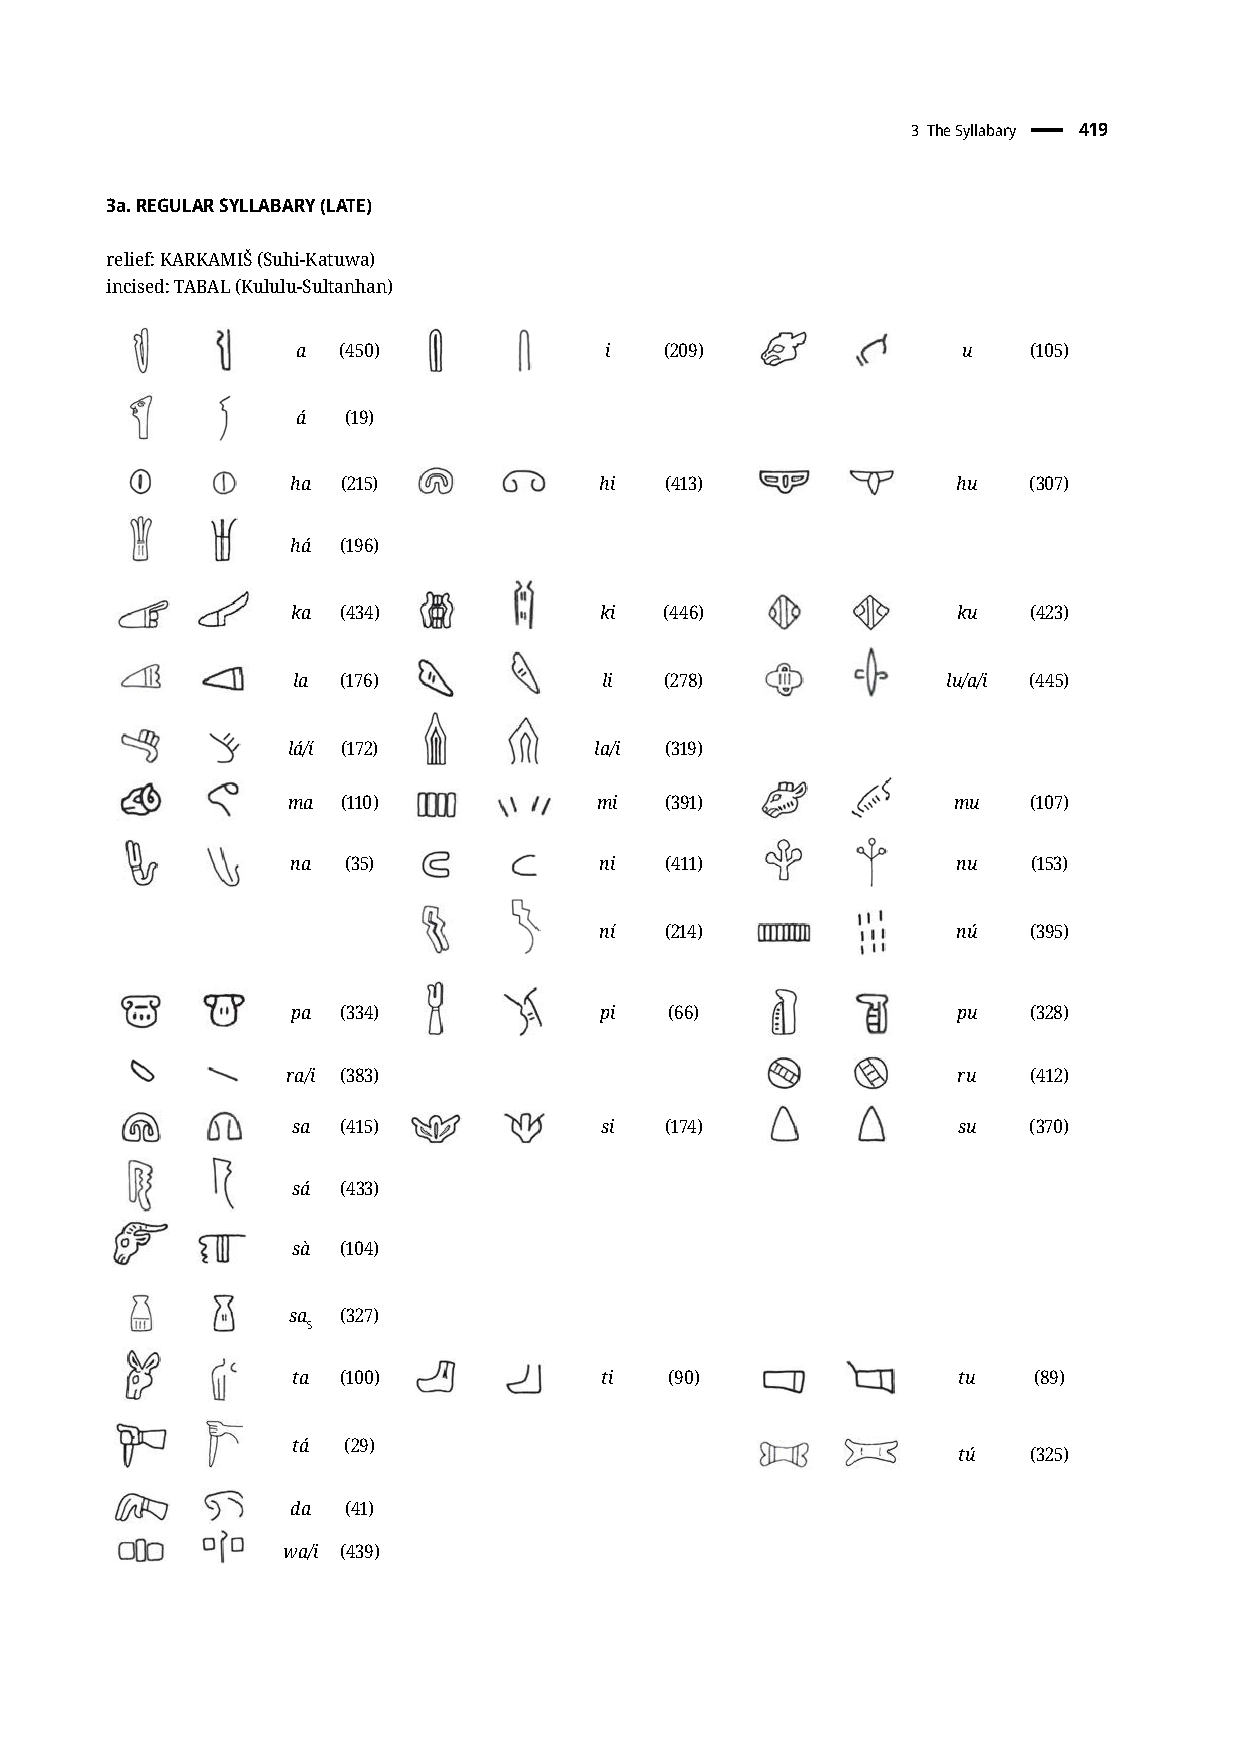
\includegraphics[width=1.2\textwidth,trim={14mm 30mm 28mm
						55mm},clip]{../../../Mídia/silaba.pdf}
		}
		\caption[Silabário regular -- Parte 1]{Silabário regular
			(\citeabbrev*{CHLI3}, p.\ 419)
			-- Parte 1}\label{tab:silabariobasico}
	\end{figure}
}
\clearpage

\clearpage
{
	\begin{figure}[ht]
		\makebox[\textwidth][r]{
			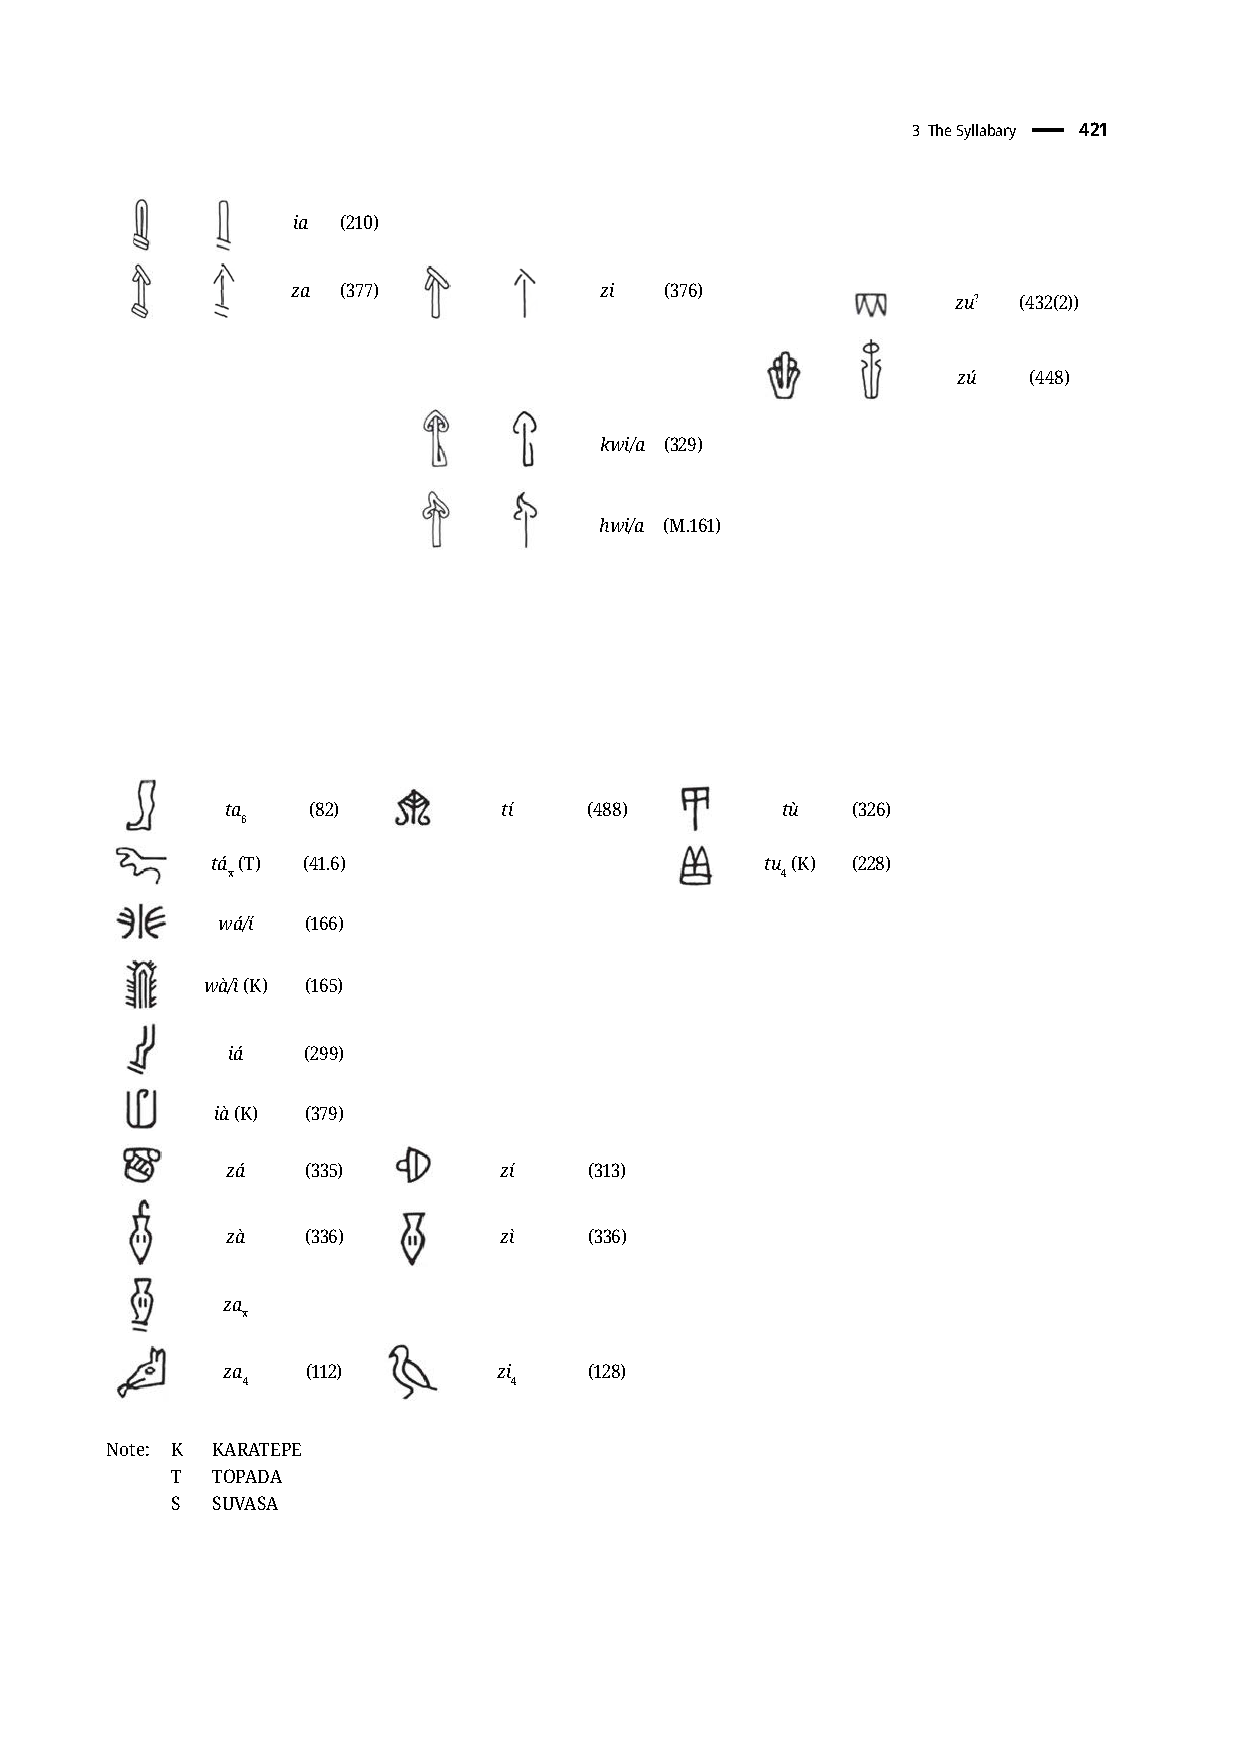
\includegraphics[width=1.2\textwidth,trim={22mm 200mm 27mm
						30mm},clip]{../../../Mídia/silabario-b.pdf}
		}
		\caption[Silabário regular -- Parte 2]{Silabário
			regular (\citeabbrev*{CHLI3}, p.\ 421)
			-- Parte 2}\label{tab:silabariobasicob}
	\end{figure}
	\begin{figure}[ht]
		\makebox[\textwidth][c]{
			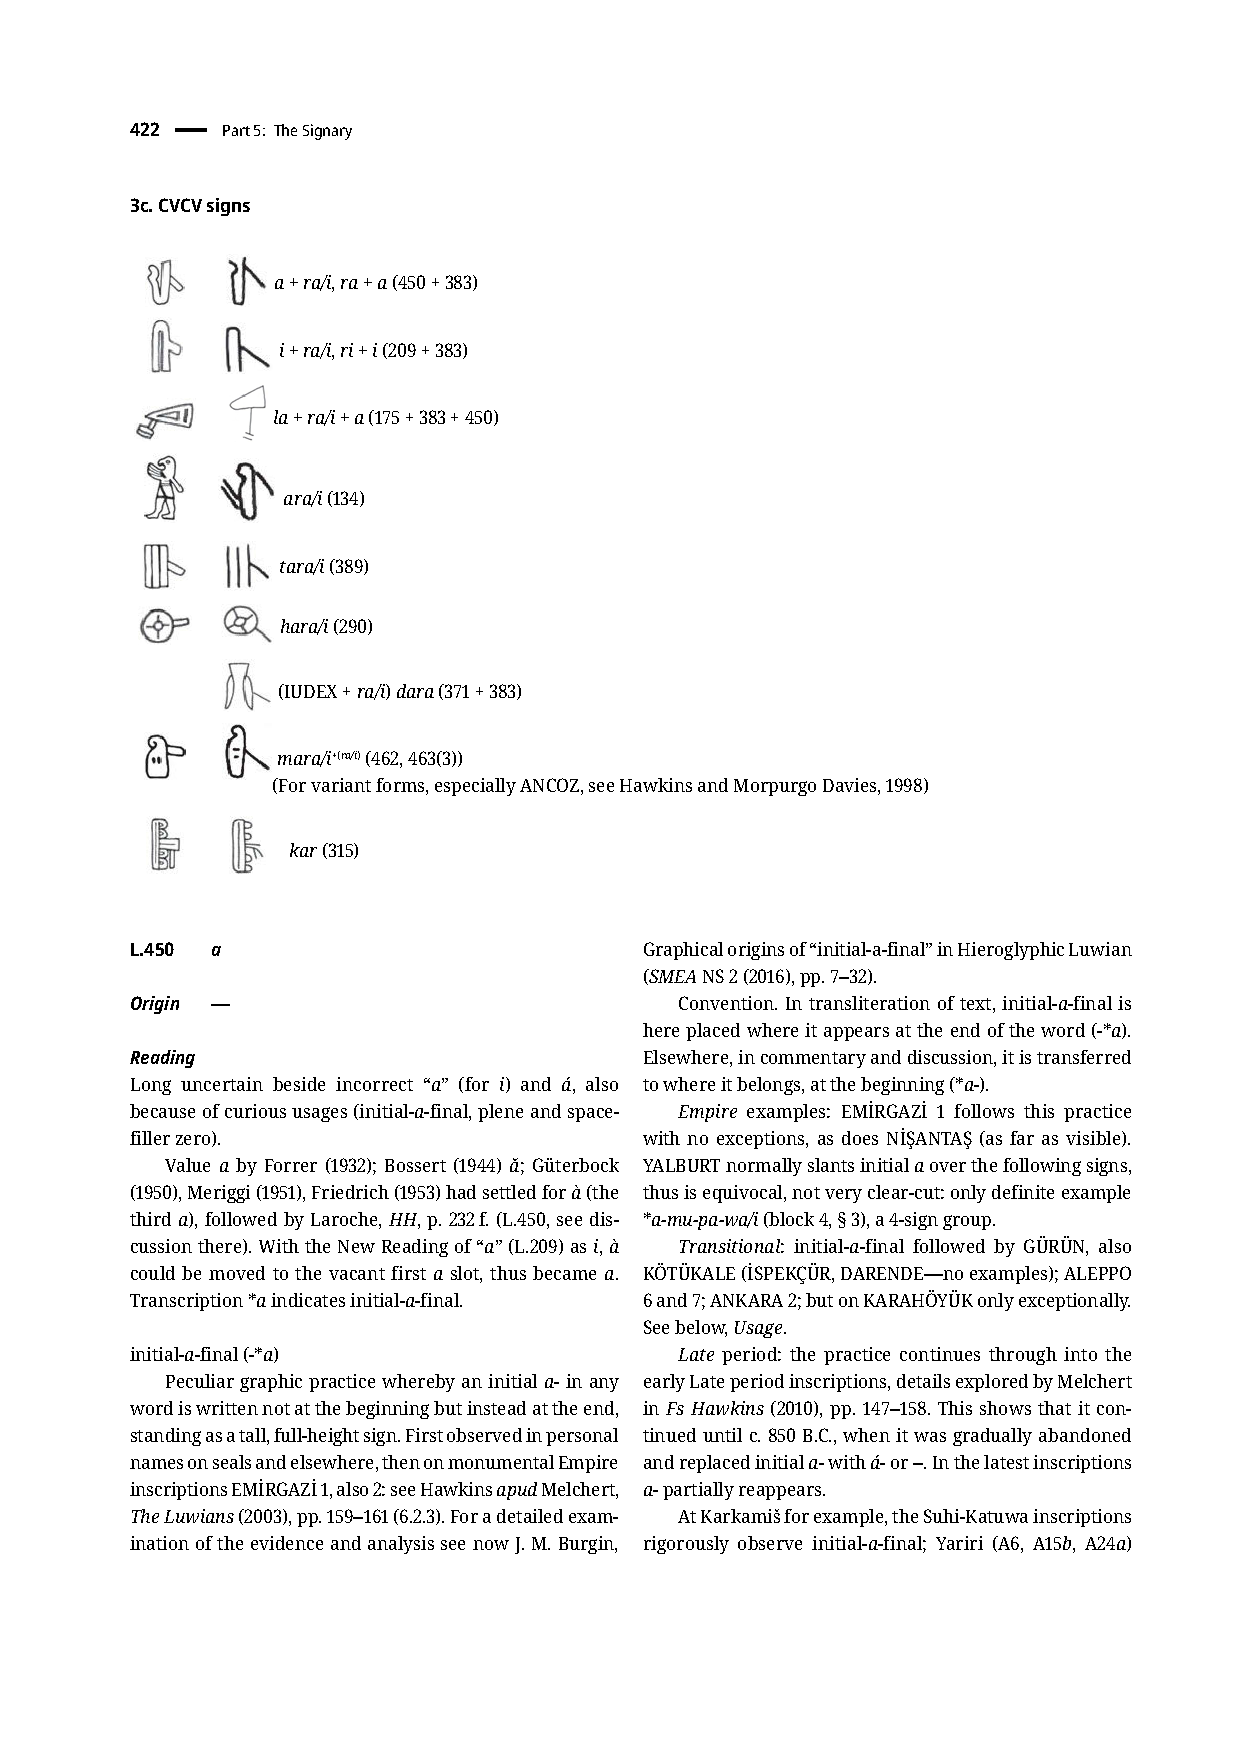
\includegraphics[width=1.1\textwidth,trim={22mm 149mm 27mm
						39mm},clip]{../../../Mídia/silabario-c.pdf}
		}
		\caption[Fonogramas CVCV]{Fonogramas CVCV~(\citeabbrev*{CHLI3}, p.\ 422)}\label{tab:CVCV}
	\end{figure}
}
\clearpage


\paragraph{Consoantes isoladas}
Com esse sistema que sempre representa sequências {(C)}V, é impossível
representar encontros consonantais e consoantes finais.
Via de regra, o costume dos escribas era de grafar uma consoante qualquer X com
o fonograma utilizado para grafar a sílaba /Xa/.
Em português, isso tornaria as palavras \emph{barco} e \emph{barraco} idênticas
na grafia, <ba-ra-co>, exigindo que o falante recuperasse pelo contexto e
conhecimento da língua qual a forma fonológica ali
representada.\footnote{Consoantes geminadas não são representadas nos
	hieróglifos anatólicos.}
Assim, para escrever \emph{hamsukalas} ``bisneto'', um escriba de MARAŞ 1 escreveu:

\exg. \ldots{} \Large 𔓷 \Large 𔒅 \Large 𔖢 \Large 𔗧 \Large 𔓊 \Large 𔗦\\
\ldots{} ha ma su ka la sá\\
\ldots{} \emph{ha\textbf{m}sukala\textbf{s}} (MARAŞ 1, §1d)

Aqui, os grafemas <ma> e <sá> devem ser interpretados como as suas respectivas
consoantes puras /m/ e /s/.

\paragraph{L.382 𔖲 ra\slash{}i} O silabograma para /ra/ ou /ri/ age de maneira
distinta dos demais por ser uma espécie de grafema \emph{enclítico}, ou seja,
ele não pode aparecer por conta própria e sempre ocorre `apoiado' em outro
fonograma.
Para representar uma sílaba final /ra/ ou /ri/, ele é representado apoiado em um
<a> ou <i>:

\ex.\a.{\Large 𔗸} = \emph{a+ra\slash{}i}
\b.{\Large 𔓰} = \emph{i+ra\slash{}i}.


\subsection{Logogramas}

Os logogramas dos hieróglifos anatólicos representam unidades de semânticas
como palavras ou conceitos que, às vezes, podem ser interpretados pelo
desenho que representam, como em~\ref{ex:ovis}.
As palavras em luvita subjacentes aos logogramas só nos são conhecidas por
ocasiões em que o escriba, além de utilizar o logograma, escreve também a
palavra com os silabogramas da forma, como é o caso em~\ref{ex:ovis-hawa}.

\exg.\label{ex:ovis}\Large 𔒇\\
OVIS\\
-\\
`ovelha' (EMİRGAZİ 1, §§19)

\exg.\label{ex:ovis-hawa}\Large 𔒇 \Large 𔓷 \Large 𔗬\\
OVIS ha wa/i\\
\emph{hawa}\\
`ovelha' (KULULU l.s. 2, §§1.2–11, etc.)


\paragraph{Forma linguística subjacente desconhecida}
No entanto, não é sempre que temos essa sorte e todas as atestações de um
logograma que nos chegaram o fizeram sem os complementos fonológicos, como
em~\ref{ex:capra}. Nesse caso, sabendo que o sinal L.104 𔑶 CAPRA é utilizado
também para grafar a sílaba /sa/, tanto na forma mais pictórica como na forma
simplificada 𔑷 e que em hitita a palavra para caprinos é \emph{šaš{(š)}a}, podemos
supor que a palavra subjacente ao logograma L.104 é \emph{sasa-}.
Comparações com o luvita cuneiforme e com línguas histórica e
geograficamente próximas do luvita hieroglífico nos permitem elucidar as formas
subjacentes que não nos chegaram grafadas, mas há casos em que é impossível
alcançar qualquer suposição razoável ou satisfatória, como em~\ref{ex:adorare}.

\exg.\label{ex:capra}\Large 𔑶\slash{}𔑷\\
CAPRA\\
\emph{sasa}{ }? (hit.\ \emph{šaš{(š)}a})\\
`cabra'


\exg.\label{ex:adorare}\Large 𔐅  \\
ADORARE\\
???\\
`rezar?' (HİSARCIK 2, § 1)

\paragraph{Logograma + silabogramas}
Como mencionado acima e ilustrado por~\ref{ex:ovis-hawa}, por vezes um logograma
é seguido da palavra subjacente escrita por completo. Essa prática é comum e
frequente.
Além disso, alguns logogramas são seguidos de silabogramas representando apenas
partes da palavra subjacente.
Por vezes, como em~\ref{ex:ponere-ha}, apenas a desinência flexional da
palavra é escrita (i.e., as marcas de caso, gênero e número para substantivos e
as de número, pessoa, tempo e modo para verbos).
Em outros casos, partes além da desinência são escritas com os silabogramas
enquanto outras são deixadas sem representação, como em~\ref{ex:ponere-wa-ta},
em que a primeira sílaba de /tu.wa.ta/, /tu/, é representada pelo logograma,
enquanto as demais sílabas são representadas com silabogramas.

\exg.\label{ex:ponere-ha}\Large 𔑇 \Large 𔓷\\
PONERE ha\\
\emph{tuwaha}\\
`(eu) coloquei' (HAMA 4, §§7)

\exg.\label{ex:ponere-wa-ta}\Large [𔑇] \Large 𔗬 \Large 𔑰\\
PONERE wa/i ta\\
\emph{tuwata}\\
`(ele) colocou' (BABYLON 3)


\noindent Nada exige que as sílabas que seguem um logograma sejam
\emph{contíguas} na palavra subjacente, por vezes apenas a primeira e última
sílabas são representadas.
A palavra para `filho', no nominativo singular, é \emph{nimuwizas}, como
atestado pela escrita plena {(FILIUS)}ni-mu-wa/i-za-sa, bastante frequente no
corpus.\footnote{KÖRKÜN, §1; KARKAMIŠ A2+3, §1; TELL AHMAR 1, §13; EĞREK, §1;
	QALʿAT EL MUDIQ, §1; HAMA 4, §1; HAMA 8, §1; HINES, §1; ŞIRZI, §1;
	KARKAMIŠ A11a, §1; TELL AHMAR 1, §§1, 19(-i).}
No entanto, em algumas inscrições, ela aparece grafada:

\exg.\Large 𔐰 \Large 𔗐 \Large 𔖪 \Large 𔗔\\
FILIUS ni za sa\\
\emph{nimuwizas} \slash{} \emph{nizas}{ }?\\
`filho' (HAMA 1–3, 6–7, §1)

É impossível decidir se a palavra subjacente nesse caso e em situações
semelhantes é uma forma realmente abreviada na fala  -- que poderia muito bem ser
uma forma coloquial -- ou se se trata apenas de uma abreviação gráfica.
Esses casos são, no entanto, raros.

\paragraph{Logogramas com múltiplas leituras}
Alguns logogramas servem para representar múltiplas palavras de um mesmo campo
semântico.
O logograma L.45 𔐰 era utilizado para denotar palavras no campo semântico de
`filho, criança, irmão', sendo transliterada pelas palavras latinas FILIUS,
INFANS e FRATER respectivamente. Nestes casos, é comum que a palavra siga
escrita também em silabogramas, ao menos parcialmente:

\ex.\ag.\Large 𔐰 \Large 𔗐 \Large 𔑿 \Large 𔗬 \Large 𔖪 \Large 𔗔\\
FILIUS ni mu wa\slash{}i za sa\\
\emph{nimuwizas} \\
`filho' (KÖRKÜN, §1)
\bg.\Large 𔐰 \Large 𔗐 \Large 𔗬𔖱 \Large 𔗐\\
INFANS ni wa\slash{}i+ra\slash{}i ni ($=$ INFANS.\emph{NI}-wa/i+ra/i-ni-?)\\
\emph{niwarani}{ }? \\
`criança (incapaz?)' (MARAŞ 4, §14)
\bg.\Large 𔐰 \Large 𔓊 \Large 𔓯 \Large 𔗐\\
FRATER la i sa ($=$ FRATER.\emph{LA}-i-sa?)\\
\emph{lanis}{ }?  ($\simeq$ luv.cun.\ \emph{nani{(ya)}-}?, cf.\ hit.\ \emph{negna-})\\
`irmão' (ALEPPO 2, §3)


\noindent Note-se que no caso de \emph{niwarani} `criança' e \emph{lani} `irmão',
não podemos estabelecer certeza da forma fonológica subjacente, posto que ou não
temos esses termos registrados em luvita cuneiforme ou o luvita cuneiforme os
registra com variações e a comparação com o hitita
é inconclusiva.\footnote{A interpretação das formas subjacentes ao logograma
	L.45 𔐰 como INFANS e FRATER discutida em~\citet[143--6]{Hawkins1980}
	e~\citet[387]{Yakubovich2010b}.}
O mesmo ocorre em diversos casos em que um logograma possui múltiplas leituras
possíveis.''

\subsection{Recomendações bibliográficas}

O panorama geral do sistema de escrita está descrito
em~\citet[p. 155ff.]{HawkinsScripts}.
Uma discussão detalhada e atualizada sobre todos os sinais conhecidos e com
as evidências utilizadas para sua interpretação pode ser encontrada
em~\citeabbrev*{CHLI3} (pp. 354--488).
Diversos artigos sobre sinais específicos são frequentemente publicados, sendo
os mais
importantes~\citet{HawkinsMorpurgoNeumann1974,Rieken2008,RiekenYakubovich2010}.

\section{Fonologia}

Utilizando apenas o silabário regular do luvita hieroglífico seríamos capazes de
reconstruir o seguinte inventário de fonemas:

\begin{compactitem}
	\item Vogais: \emph{a}, \emph{i}, \emph{u}
	\item Oclusivas: \emph{p}, \emph{t}, \emph{k}
	\item Nasais: \emph{m}, \emph{n}
	\item Fricativas: \emph{s}, \emph{z}, \emph{h}
	\item Outras: \emph{r}, \emph{l}, \emph{w}, \emph{y}
\end{compactitem}
No entanto, esse inventário de fonemas não parece ser o inventário realmente
utilizado pela língua.

\subsection{Vogais}

\paragraph{Vogais longas}
O cuneiforme utilizado para grafar o luvita cuneiforme é capaz de representar
a oposição entre vogais longas e
breves por meio da grafia \emph{plena}, quando a vogal longa é representada pela
adição do cuneiforme representando a vogal sem consoantes.
Os escribas não se valem da escrita plena de maneira regular, mas alguns pares
contrastivos, como~\Next, apontam para uma distinção fonêmica.

\ex.\ag.\foreignlanguage{hittite}{𒀀} \foreignlanguage{hittite}{𒀜}
\foreignlanguage{hittite}{𒁺}  \foreignlanguage{hittite}{𒉿}
\foreignlanguage{hittite}{𒀀}  \foreignlanguage{hittite}{𒀠}\\
\textbf{a}- \textbf{ad}- du- \textbf{wa}- \textbf{a}- \textbf{al}\\
\emph{\textbf{ād}du\textbf{wāl}}\\
`mal' (88 II 11, \emph{KBo} XXIX 9 Ro 10*)
\bg.\foreignlanguage{hittite}{𒀀} \foreignlanguage{hittite}{𒀜}
\foreignlanguage{hittite}{𒁺}  \foreignlanguage{hittite}{𒉿}
\foreignlanguage{hittite}{𒆷}\\
\textbf{a}- \textbf{ad}- du- wa- la\\
\emph{\textbf{ād}duwala}\\
`males' (39 iii 26.)\footnote{Exemplos tirados de~\citet{Melchert1993}.}

\paragraph{Escrita do /a/ inicial} Por razões ainda desconhecidas, o /a/ em
início de palavra com frequência aparece grafado no final da palavra,
vide~\Next. Para deixar claro que este é o caso, pode-se transliterar um <a>
inicial escrito em posição final com um asterisco.
Essa prática parece mais comum na idade do bronze, mas não deixa de ser
utilizada ao longo de todo o uso do sistema de escrita.
Há ainda casos em que o /a/ em início de sentença não é grafado.

\exg.\Large 𔗔 \Large  𔑢 \Large 𔗷\\
sa tu a\\
*\emph{asatu}\\
`que ele seja' (EMİRGAZİ, §17)



\subsection{Oclusivas}

\paragraph{/t/ vs. /d/}
Em primeiro lugar, temos como evidência o \emph{rotacismo} de algumas dentais em
ambiente intervocálico.
O rotacismo não ocorre de maneira consistente em nenhuma região geográfica ou
período da língua luvita e formas com os sinais para /t/ e /r/ com frequência
aparecem no mesmo texto.
As formas que sofrem rotacismo são, de acordo
com~\citet[249--50]{MorpurgoDavies1982}:

\begin{compactenum}
	\item desinências de ablativo em \emph{-adi}: <\emph{-a-ti}> e
	<\emph{-Ca-ra\slash{}i-{(i)}}>.
	\item desinências de terceira pessoa:
	\begin{compactenum}
		\item presente \emph{-di}: <\emph{-ti}> ou <\emph{-ra\slash{}i-{(i)}}>;
		\item pretérito \emph{-da}: <\emph{-ta}> ou <\emph{-ra\slash{}i}>;
		\item imperativo \emph{-du}: <\emph{-tu}> ou <\emph{-ru}>.
	\end{compactenum}
	\item partículas enclíticas:
	\begin{compactenum}
		\item reflexivo / pronominal \emph{=di}: <\emph{-ti}> ou <\emph{-ra\slash{}i-{(i)}}>;
		\item pronominal \emph{=du}: <\emph{-tu}> ou <\emph{-ru}>;
		\item pronominal \emph{=ada}: <\emph{-a-ta}> ou <\emph{-a+ra\slash{}i}>.
	\end{compactenum}
	\item itens lexicais, dois deles com etimologia bem estabelecida:
	\begin{compactenum}
		\item <\emph{á-ru-na}> `comer' de \textsc{pie} *\emph{ed-};
		\item <\emph{pa+ra\slash{}i-za}> (dat.pl., SULTANHAN, §9) de
		\textsc{pie} *\emph{ped-}, mas também grafado <\emph{pa-da}> (dat.sg.,
		SULTANHAN, §6).
	\end{compactenum}
\end{compactenum}
Por comparação com a evidência do luvita cuneiforme\footnote{Em luvita
	cuneiforme, embora irregular, a consoante /d/ é representada pela grafia das
	dentais sem geminação, como \emph{a-a-ta} /ada/ `ele fez', em contraste com
	\emph{a-at-ta} /ata/ (conj.+partic.).}
e lício e por razões tipológicas, assume-se atualmente que o rotacismo apenas
incindia sobre uma consoante próxima de uma oclusiva sonora dental
/d/.\footnote{Esse /d/ pode ter duas origens, como
	argumenta~\textcite{MorpurgoDavies1982}:
	\begin{inparaenum}
		\item \textsc{pie} *\emph{d};
		\item \textsc{pie} *\emph{t} em pelo menos dois contextos:
		\begin{inparaenum}
			\item \textsc{pie} V̄́tV > luv.com.\ V̄́dV;\@
			\item \textsc{pie} V́CVtV > luv.com.\ V́CVdV;\@
		\end{inparaenum}
	\end{inparaenum}
	i.e., após vogais longas ou ditongos acentuados e entre vogais não acentuadas.
}
Além disso, os sinais previamente considerados intercambiáveis da série
/ta/, antigos <ta\textsubscript{1-5}>, deixaram de sê-lo desde o artigo
de~\citet{Rieken2008}, que demonstrou que <ta\textsubscript{3}> não é
intercambiável com <ta\textsubscript{1--2}> e desde o artigo
de~\citet{RiekenYakubovich2010}, que demonstrou que os antigos
<ta\textsubscript{4}> e <ta\textsubscript{5}> correspondem a <la\slash{}i> e
<lá\slash{}í>, respectivamente.

\paragraph{/p/ vs. /b/ e /k/ vs. /g/}
Por comparação com o luvita cuneiforme, cujo sistema de
escrita diferencia oclusivas surdas e sonoras, ainda que os escribas não
registrem a oposição de maneira sistemática ou regular, pode-se supor que o
luvita diferenciava também surdas e sonoras para as oclusivas bilabiais e
velares.
Por vezes utiliza-se outras línguas que tiveram contato com o luvita para
decidir se um sinal /CV/ representa uma C surda ou sonora, como no caso do
exemplo em~\Next: a divindade <KuPaPa> parece corresponder à mesma
divindade referida pelo assírio antigo \emph{\textsuperscript{D}Ku-ba-ba},
pelas formas hititas \emph{\textsuperscript{D}ku-ba-ba-},
\mbox{\emph{\textsuperscript{D}ku-pa-pa}} e \emph{\textsuperscript{D}ku-pa-wa},
hurrita e aramaico \emph{kbb} e, talvez, pelo grego Κυβήβη.\footnote{%
	Hdt. 5.102, possivelmente a forma grega foi intermediada pelo lídio
	\emph{kufad} (4a4).
	A associação com o grego Κυβέλη (Ar. Av. 876), com o frígio
	\emph{(matar) Kubileya} (B-01), \mbox{\emph{(matar) Kubeleya}} (\mbox{W-04})
	é problemática, vide \citet[280--1]{Obrador2020} e \citet{Oreshko2021},
	que disputa inclusive a associação com a forma grega Κυβήβη.
}


\exg.\Large 𔖖 \Large 𔗜 \Large 𔕸 \Large 𔕸\\
DEUS ku pa pa\\
(DEUS)\emph{Kubaba} \\
Kubaba


\subsection{Nasais}

\paragraph{/n/ pré\hyp{}consonantal}
Uma particularidade da escrita luvita é não grafar o /n/
pré\hyp{}consonantal onde ele seria esperado pela reconstrução linguística ou
comparação com o luvita cuneiforme.\footnote{%
	Alguns interpretam nisso um sinal de que, ao menos no dialeto das inscrições
	em hieróglifos, os falantes não mais produziam a consoante /n/, mas sim
	a nasalização da vogal anterior, o que não estaria documentado nos textos
	luvitas em cuneiforme por conta ou de práticas ortográficas de escribas
	acostumados com a ortografia cuneiforme do hitita, ou de uma diferença
	dialetal entre o dialeto da era do bronze e da era do ferro. Se for este o
	caso, o exemplo~\ref{ex:tatinzi} representaria /ta.tĩ.tsi/.}
Em português, isso tornaria as palavras \emph{manga} e \emph{maga} idênticas na
grafia, <ma-ga>.
Para escrever a palavra para `pais', grafa-se:

\exg.\label{ex:tatinzi}\Large 𔐞 \Large 𔑣 \Large 𔖩\\
tá ti zi\\
\emph{tati\textbf{n}zi}  (MARAŞ 1, §12)



\subsection{Recomendações bibliográficas}

Sobre a fonologia histórica do luvita em relação às demais línguas anatólicas,
ver~\citet[p. 229ff.]{Melchert1994}.
Para uma descrição detalhada do sistema fonológico luvita,
ver~\citet[p. 177ff.]{MelchertLanguage}.
A tese de~\citet{Vertegaal2020} contém discussões sobre a grafia de dentais e
vogais longas em luvita.

\section{Flexão nominal}

Os substantivos, adjetivos e pronomes em luvita podem flexionar em gênero (Comum e Neutro),
número (Singular e Plural) e caso (Nominativo, Acusativo, Genitivo, Dativo e
Ablativo).
Pronomes não possuem o sistema de caso completo e por vezes não possuem
distinção de gênero.
As desinências utilizadas na maioria dos contextos são:

\begin{center}
	\begin{tabular}[c]{llll}
		\toprule
		                      & \Sg{}\emph{}             &                       & \Pl{}\emph{}                   \\
		\midrule
		\Nom{} \Com{}         & \emph{-s}                & \Nom{} \Com{}         & \multirow{2}{4em}{\emph{-nzi}} \\
		\Acu{} \Com{}         & \emph{-{(a)}n}           & \Acu{} \Com{}         &                                \\
		\Nom{}/\Acu{} \Neut{} & \emph{-n, ∅}             & \Nom{}/\Acu{} \Neut{} & \emph{-a{(ya)}}                \\
		\Gen{}                & \emph{-{(a)}s, -{(a)}si} &                       &                                \\
		\Dat{}                & \emph{-i{(ya)}, -a, -an} & \Dat{}                & \emph{-anza}                   \\
		\Abl{}                & \emph{-adi}              & \Abl{}                & \emph{-adi}                    \\
		\bottomrule
	\end{tabular}
\end{center}

Por conta das idiossincrasias do sistema de escrita hieroglífico, todas as
desinências terminadas em consoantes são grafadas com o sinal correspondente à
consoante C em questão na série do /a/, ou seja, <Ca>.
Outras particularidades dos sistema de flexão nominal do luvita incluem:
\begin{compactitem}
	\item o gênero neutro não diferencia nominativo de acusativo
	\item os casos nominativo e acusativo neutro singular costumam ser seguidos de
	uma partícula \emph{-sa\slash{}za}, sendo assim duplamente
	marcados\footnote{É possível que essa forma tenha sido derivada do pronome
		demonstrativo \emph{za-} `este, esta', mas ainda não está claro em quais
		contextos a partícula aparece e sua história. Em cuneiforme, há uma passagem
		em que o valor de demonstrativo está preservado: \emph{īzagan=za\ldots{}
			šapiyaimman} `este \emph{i.} está \emph{s.}-ado' Kbo 29.6 Ro 25.}
	\item o gênero comum não diferencia nominativo de acusativo no plural
	\item o caso genitivo não é capaz de expressar pluralidade do possessor
	\item o caso genitivo compete com os adjetivos possessivos em
	\emph{-asa\slash{}i}
	\item a desinência \emph{-an} do dativo ocorre só em adjetivos possessivos
	em \emph{-asa\slash{}i}
	\item o caso ablativo não diferencia singular de plural
\end{compactitem}

\subsection{Substantivos}

Dada a situação fragmentária da língua, não temos o paradigma
completo de flexão de nenhum substantivo ou adjetivo. A tabela a seguir contém
as formas para o substantivo de gênero comum \emph{huha-} `avô', suplementada
onde necessário por \emph{ziti-} `homem', \emph{hawi-} `ovelha', \emph{tarkasna\slash{}i-}
`burro' e \emph{masani-} `deus' e o neutro é representado por \emph{kuwalan-}
`exército' e \emph{katin{(a)}-} `vasilha'.


\begin{center}
	\begin{tabular}[c]{lll}
		\toprule
		                      & \Sg{}\emph{}                  & \Pl{}\emph{}                       \\
		\midrule
		\Nom{} \Com{}         & \emph{huha-s}                 & \multirow{2}{4em}{\emph{huha-nzi}} \\
		\Acu{} \Com{}         & \emph{huha-n}                 &                                    \\
		\Nom{}/\Acu{} \Neut{} & \emph{kuwalan=za}             & \emph{katina}                      \\
		\Gen{}                & \emph{ziti-s}, \emph{hawi-si} &                                    \\
		\Dat{}                & \emph{huha}                   & \emph{tarkasniy-anza}              \\
		\Abl{}                & \emph{huh-adi}                & \emph{masan-adi}                   \\
		\bottomrule
	\end{tabular}
\end{center}


\subsection{Adjetivos}
A seguir, a declinação dos adjetivos, utilizando a forma \emph{tati{(ya)}-}
`paterno\slash{}a', suplementada por \emph{tarawani-} `justo',
\emph{hanti{ya}-} `primeiro' e do adjetivo possessivo \emph{lanisa-} `do irmão'.

\begin{center}
	\begin{tabular}[c]{lll}
		\toprule
		                      & \Sg{}\emph{}                 & \Pl{}\emph{}                       \\
		\midrule
		\Nom{} \Com{}         & \emph{tarawani-s}            & \multirow{2}{4em}{\emph{tati-nzi}} \\
		\Acu{} \Com{}         & \emph{tarawani-n}            &                                    \\
		\Nom{}/\Acu{} \Neut{} & \emph{tatiya-n=za}           & \emph{tati-ya}                     \\
		\Gen{}                & \emph{tarawani-s}            &                                    \\
		\Dat{}                & \emph{tati}, \emph{lanisa-n} & \emph{tati-nza}                    \\
		\Abl{}                & \emph{hantiy-ari}            & \emph{tatiy-adi}                   \\
		\bottomrule
	\end{tabular}
\end{center}


\subsection{Pronomes}

\subsubsection{Pronomes pessoais}

\paragraph{Formas tônicas}
Os pronomes pessoais tônicos -- também chamados de
ortotônicos -- não possuem formas de genitivo e seu paradigma é bastante
incompleto. A terceira pessoa não possui um pronome pessoal dedicado, sendo
utilizado o demonstrativo \emph{apa-} `aquele' no lugar.


\begin{center}
	\begin{tabular}[c]{lll|ll}
		\toprule
		       & 1\Sg{}\emph{} & 1\Pl{}\emph{}      & 2\Sg{}\emph{} & 2\Pl{}\emph{}                          \\
		\midrule
		\Nom{} & \emph{amu}    & \emph{anzunz{(a)}} & \emph{ti}     & \emph{unzunz{(a)}}, \emph{unzuns{(a)}} \\
		\Acu{} & \emph{amu}    & {?}\emph{}         & \emph{tu}     & {?}\emph{}                             \\
		\Dat{} & \emph{amu}    & {?}\emph{}         & \emph{tu}     & {?}\emph{}                             \\
		\Abl{} & {?}\emph{}    & {?}\emph{}         & \emph{tuwati} & \emph{unzati}                          \\
		\bottomrule
	\end{tabular}
\end{center}

\noindent Alguns detalhes sobre as formas tônicas dos pronomes pessoais:
\begin{compactitem}
	\item \emph{amu} pode ser grafado \emph{mu} por aférese
	\item \emph{tuwati} e \emph{unzati} podem ser formas de possessivos
	\item o silabograma para <zu>, L.432 𔗥, das formas plurais tem leitura disputada,
	sobretudo para os textos da idade do ferro, \citet[65--68]{Yakubovich2010}
	propõe <za\textsubscript{x}>.
\end{compactitem}

\paragraph{Formas clíticas}
Os pronomes pessoais também possuem formas átonas que se
comportam de maneira clítica (apoiados fonologicamente na primeira palavra da
sentença).
Estes pronomes não diferenciam caso, são utilizados no lugar de nominativos,
acusativos e dativos e por vezes aparecem junto da forma tônica.

\begin{center}
	\begin{tabular}[c]{lll|ll}
		\toprule
		                           & 1\Sg{}\emph{} & 1\Pl{}\emph{} & 2\Sg{}\emph{}   & 2\Pl{}\emph{} \\
		\midrule
		\Nom\slash\Acu\slash\Dat{} & \emph{=mu}    & \emph{=anza}  & \emph{=du, =di} & \emph{=manza} \\
		\bottomrule
	\end{tabular}
\end{center}


\paragraph{Clíticos de terceira pessoa}
A terceira pessoa possui uma série de clíticos próprios com distinção de caso em
parte do paradigma:

\begin{center}
	\begin{tabular}[c]{lll}
		\toprule
		                      & 3\Sg{}\emph{} & 3\Pl{}\emph{} \\
		\midrule
		\Nom{}\Com{}          & \emph{=as}    & \emph{=ada}   \\
		\Acu{}\Com{}          & \emph{=an}    & \emph{=ada}   \\
		\Nom\slash\Acu\Neut{} & \emph{=ada}   & \emph{=ada}   \\
		\Dat{}                & \emph{=du}    & \emph{=manza} \\
		\bottomrule
	\end{tabular}
\end{center}

\paragraph{Pronomes reflexivos}
Todas as formas de pronomes reflexivos são enclíticas.

\begin{center}
	\begin{tabular}[c]{ll|ll|ll}
		\toprule
		1\Sg{}\emph{} & 1\Pl{}\emph{} & 2\Sg{}\emph{} & 2\Pl{}\emph{} & 3\Sg{}\emph{} & 3\Pl{}\emph{} \\
		\midrule
		\emph{=mi}    & \emph{=anza}  & \emph{=di}    & \emph{=manza} & \emph{=di}    & \emph{=manza} \\
		\bottomrule
	\end{tabular}
\end{center}

\subsubsection{Possessivos}

\subsubsection{Demonstrativos}
As formas dos pronomes demonstrativos são \emph{za-} `esse, este' e
\emph{apa\slash{}i-} `aquele'.
Formas adverbiais também são formadas a partir dos temas dos demonstrativos,
como \emph{zati} `aqui' e \emph{apati} `ali'.

\paragraph{za- `esse/este'}

\begin{center}
	\begin{tabular}[c]{lll}
		\toprule
		                 & \Sg{}\emph{}     & \Pl{}\emph{}                    \\
		\midrule
		\Nom{} \Com{}    & \emph{zas}       & \multirow{2}{4em}{\emph{zanzi}} \\
		\Acu{} \Com{}    & \emph{zan}       &                                 \\
		\Nom/\Acu\Neut{} & \emph{za}        & \emph{zaya}                     \\
		\Gen{}           & \emph{zas, zasi} &                                 \\
		\Dat{}           & \emph{zati}      & \emph{zatanza, zatiyanza}       \\
		\Abl{}           & \emph{zin}       & \emph{}                         \\
		\bottomrule
	\end{tabular}
\end{center}

\paragraph{apa- `aquele'}

\begin{center}
	\begin{tabular}[c]{lll}
		\toprule
		                 & \Sg{}\emph{}       & \Pl{}\emph{}                             \\
		\midrule
		\Nom{} \Com{}    & \emph{apas, apis}  & \multirow{2}{4em}{\emph{apanzi, apinzi}} \\
		\Acu{} \Com{}    & \emph{apan, apin}  &                                          \\
		\Nom/\Acu\Neut{} & \emph{apa}         & \emph{apaya}                             \\
		\Gen{}           & \emph{apas, apasi} &                                          \\
		\Dat{}           & \emph{apati}       & \emph{apatanza}                          \\
		\Abl{}           & \emph{apin}        & \emph{}                                  \\
		\bottomrule
	\end{tabular}
\end{center}

\subsubsection{Pronome interrogativo e relativo}

A forma \emph{kwi\slash{}a-} é sempre escrita com o logograma L.329 𔕰 REL\@ e
é utilizada tanto com o valor relativo como com o valor interrogativo.
O redobro, \emph{kwis kwis} ou \emph{kwis ima kwis}, é utilizado para dar o
sentido `quem quer que', também produzido pela forma indefinida \emph{kwis=ha}.

\begin{center}
	\begin{tabular}[c]{lll}
		\toprule
		                 & \Sg{}\emph{}       & \Pl{}\emph{}                     \\
		\midrule
		\Nom{} \Com{}    & \emph{kwis}        & \multirow{2}{4em}{\emph{kwinzi}} \\
		\Acu{} \Com{}    & \emph{kwin}        &                                  \\
		\Nom/\Acu\Neut{} & \emph{kwa{(n)}=za} & \emph{kwaya}                     \\
		\Dat{}           & \emph{kwati}       & \emph{kwatanza}                  \\
		\Abl{}           & \emph{?}           & \emph{}                          \\
		\bottomrule
	\end{tabular}
\end{center}

\noindent Derivados desse pronome são:
\begin{compactitem}
	\item advérbios \emph{kwitan} `onde (quer que)' e \emph{kwipa} `de fato'
	\item as conjunções:
	\begin{compactitem}
		\item \emph{kwari} `porque, uma vez que, como, se, quando'
		\item \emph{kwati} `se, de modo que'
		\item \emph{kwa{(n)}za} `uma vez que, porque, embora'
		\item \emph{kwi} `muito embora, enquanto'
	\end{compactitem}
\end{compactitem}


\clearpage

\section{Leitura: BABYLON 3}

Trata-se de um vaso em estado fragmentário (\autoref{fig:babylon3}) escavado por
Koldewey na década de 20 onde se acredita ser a cidade de Babilônia, sítio
arqueológico de Arpada, noroeste de Alepo, contendo uma inscrição no
beiral em cursivas de baixo relevo, sentido sinistroverso, em duas linhas a
serem lidas em conjunto (para cada coluna, lê-se o caractere na primeira linha,
em seguida o da segunda linha e assim sucessivamente).
A inscrição, embora escavada na Babilônia, provavelmente teria sido
produzida em Alepo e lá dedicada ao deus do trovão Tarhunta da cidade, o que é
indicado pelo epíteto 𔓢𔑞𔕸𔗐 \textsc{tonitrus.halpa}-\textit{pa-ni}
= \textit{halpa{(wa)}ni} `halabeu'. Desde o período imperial,
a combinação dos logogramas L.199+L.84 \slash{} 85 𔓢𔑝\slash{}𔑞
\textsc{tonitrus+crus$_2$ \slash{} genuflectere}
via de regra denota a cidade de Halab.\footnote{Com L.84
\textsc{crus}$_2$ 𔑝: ALEPPO 5; NİŞANTEPE 2, no. 57; İMAMKULU.\@
Com L.85 \textsc{genuflectere} 𔑞:  ALEPPO 6; TELL AHMAR 5;
KÖRKÜN;\@ BABYLON 1; BABYLON 3; \mbox{HAMA 1}.\@
Também nomes próprios de figuras associadas a Halab são grafados com essa
combinação, como Halparuntiya em
MARAŞ 1 \textsc{tonitrus.halpa}-\textit{pa-ru-ti{(-i)}-ia-}.
}
A data de produção é incerta, mas deve cair entre o século IX e VIII
\textsc{aec}.

\vfill

\begin{figure}[!htb]
	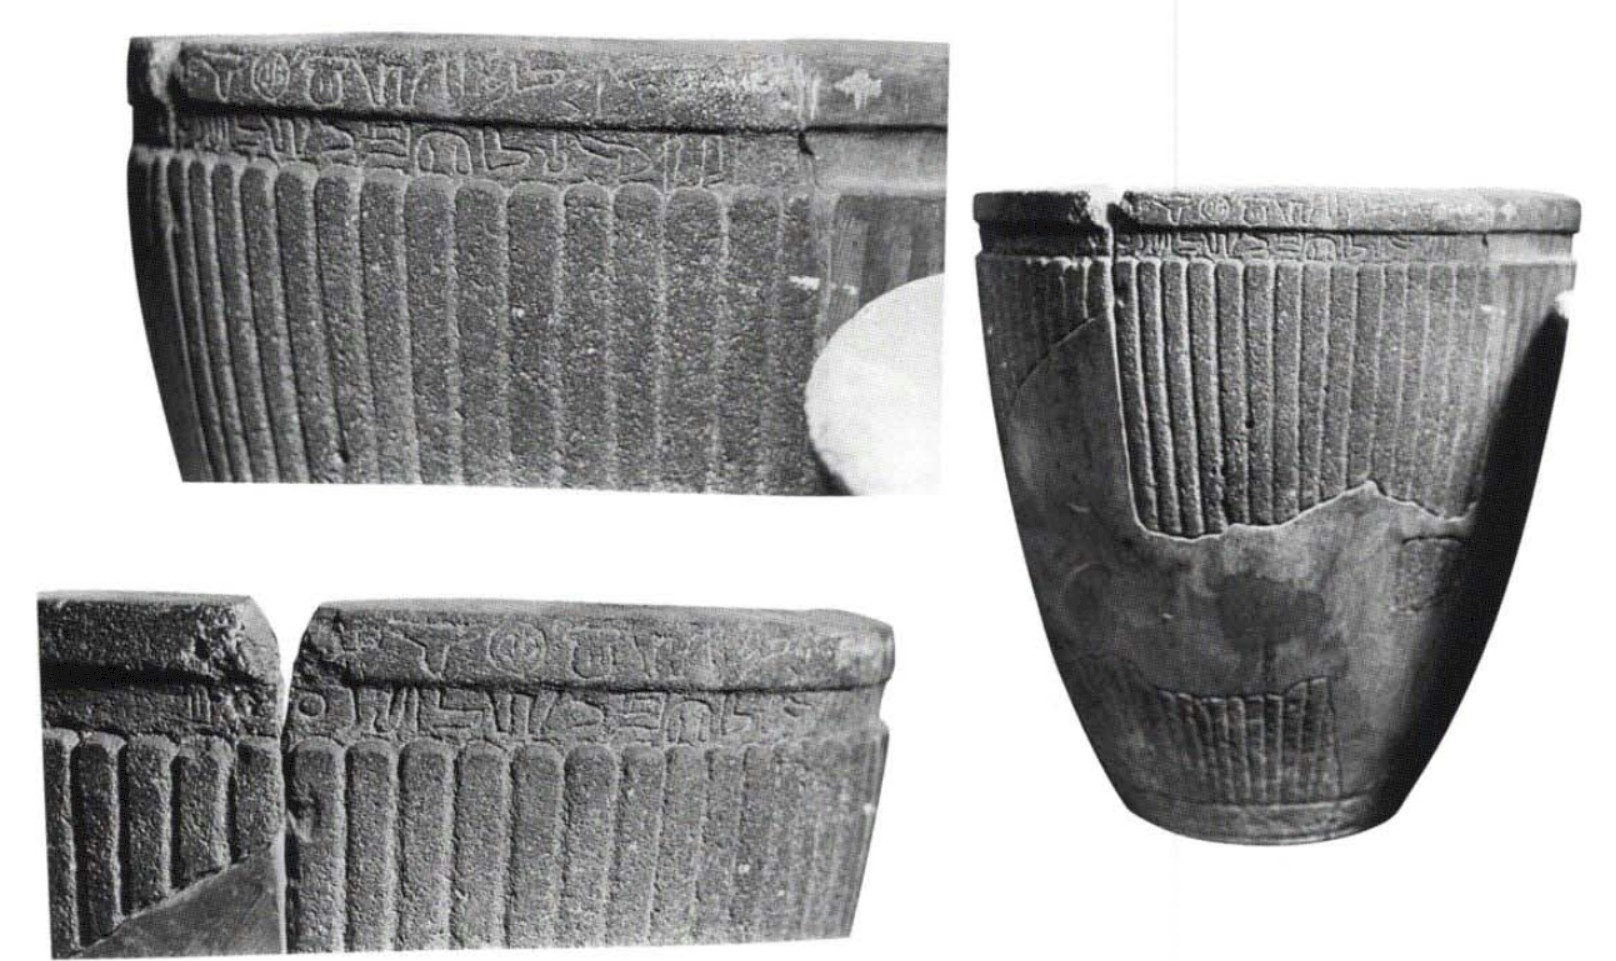
\includegraphics[width=\textwidth,trim={4mm 2mm 12mm 11mm},clip]{../../../Mídia/aleppo23.jpg}
	\caption[BABYLON 3]{
		BABYLON 3. Diâmetro: 0.66m.; Profundidade
		(interna): 0.67m. Imagens produzidas e traçado feito por
		\citeabbrev*{CHLI13} (\emph{plate} 212). Atualmente no
		\foreignlanguage{german}{Vorderasiatisches Museum}, Berlin,
		no. VA Bab. 1507.
	}\label{fig:babylon3}
\end{figure}

\clearpage

\begin{center}
	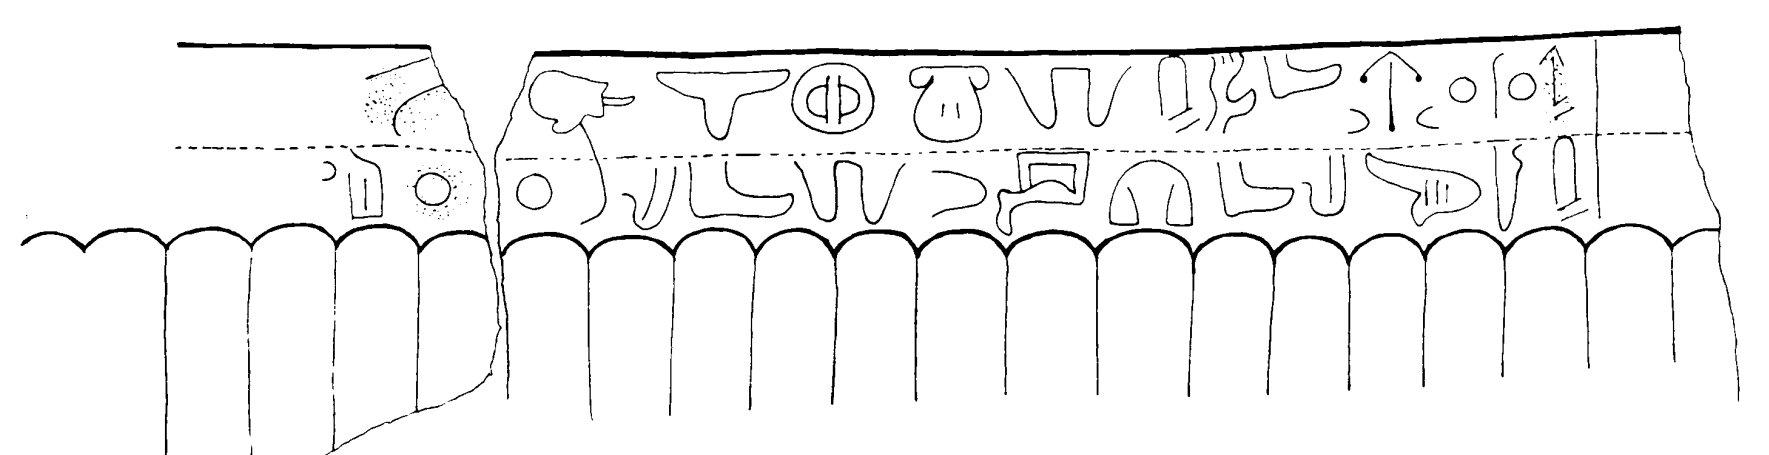
\includegraphics[width=\textwidth,trim={100mm 60mm 55mm 10mm},clip]{../../../Mídia/babylon3.png}
\end{center}
\exg.{\Large 𔖪𔓱𔗬𔗷} {\Large 𔗎𔔯𔗏𔗧𔑣𔐤} {\Large 𔑵𔑣𔓱𔗔} {\Large 𔓢𔑞𔕸𔗐} {\Large 𔖖𔓢𔕙𔑣}
{\Large 𔐎𔐤} {\Large [𔑇]𔗬𔑰}\\
za-ia-wa\slash{}i-a\hspace{10pt} ``SCALPRUM''-ka-ti-na\hspace{10pt}
CERVUS\textsubscript{2}-ti-ia-sa\hspace{10pt} TONITRUS.HALPA-pa-ni\hspace{10pt}
DEUS.TONITRUS-hu-ti\hspace{10pt} PRAE-na\hspace{10pt} [PONERE]-wa/i-ta\\
zaya=wa katina Runtiyas halpawani Tarhunti paran tuwada

\exg.zaya=wa katina Runtiyas halpawani Tarhunti paran tuwada\\
\Det{}\Acu{}\Pl{} vasilha.\Neut{}\Acu{}\Pl{} R.\Com{}\Nom{}\Sg{} halabeu.\Com{}\Dat{}\Sg{} T.\Com{}\Dat{}\Sg{} \Prep{} colocar-3\Sg\\
Estes vasos Runtiya dedicou ao Tarhunta halabeu.




\hspace{10pt}
\begin{multicols}{2}[\noindent\textbf{Vocabulário}]
	\begin{hangparas}{1em}{1}
		\raggedright%
		\textbf{\emph{halpawani}-} (\emph{adj.}) \tabto{1em} proveniente de Halpa \tabto{1em} halabeu\\
		\textbf{\emph{katina}-} (\emph{subst.neut.}) \tabto{1em} vaso, vasilha\\
		\textbf{\emph{paran}} (\emph{prep.}) \tabto{1em} em frente a\\
		\textbf{\emph{Runtiya}-} (NP) \tabto{1em} Runtiya\\
		\textbf{\emph{Tarhunta}-} (TE) \tabto{1em} Tarhunta\\
		\textbf{\emph{tuwa}-} (\emph{v.t.}) \tabto{1em} colocar\\
	\end{hangparas}
\end{multicols}


\backmatter%

\printbibliography%

\end{document}
